\documentclass[compress,red]{beamer}
\mode<presentation>

\usepackage{etex}
\setbeamertemplate{navigation symbols}{}
\usepackage{pgfpages}

\usetheme{Warsaw}

% define your own colors:
\definecolor{Red}{rgb}{1,0,0}
\definecolor{Blue}{rgb}{0,0,1}
\definecolor{Green}{rgb}{0,1,0}
\definecolor{magenta}{rgb}{1,0,.6}
\definecolor{lightblue}{rgb}{0,.5,1}
\definecolor{lightpurple}{rgb}{.6,.4,1}
\definecolor{gold}{rgb}{.6,.5,0}
\definecolor{orange}{rgb}{1,0.4,0}
\definecolor{hotpink}{rgb}{1,0,0.5}
\definecolor{newcolor2}{rgb}{.5,.3,.5}
\definecolor{newcolor}{rgb}{0,.3,1}
\definecolor{newcolor3}{rgb}{1,0,.35}
\definecolor{darkgreen1}{rgb}{0, .35, 0}
\definecolor{darkgreen}{rgb}{0, .6, 0}
\definecolor{darkred}{rgb}{.75,0,0}

\xdefinecolor{olive}{cmyk}{0.64,0,0.95,0.4}
\xdefinecolor{purpleish}{cmyk}{0.75,0.75,0,0}


\useoutertheme[subsection=false]{smoothbars}


% include packages
\usepackage{todonotes}
\presetkeys{todonotes}{inline}{}
\usepackage{subfigure}
\usepackage{multicol}
\usepackage{amsmath}
\usepackage{epsfig}
\usepackage{graphicx}
\usepackage[all]{xy}
\usepackage{url}
\usepackage{multimedia}
\usepackage{hyperref}
\usepackage{helvet}
\usepackage[polish,english]{babel}
\usepackage[utf8]{inputenc}
\usepackage{multirow}
\usepackage{pgfpages}

\newcommand{\backupbegin}{
   \newcounter{framenumberappendix}
   \setcounter{framenumberappendix}{\value{framenumber}}
}
\newcommand{\backupend}{
   \addtocounter{framenumberappendix}{-\value{framenumber}}
   \addtocounter{framenumber}{\value{framenumberappendix}} 
}

\graphicspath{ {../../figures/} }


\title[White Rabbit \hspace{2em}\insertframenumber/\inserttotalframenumber]
{The White Rabbit project\\ \small an Ethernet-based solution for sub-ns synchronization and deterministic delivery}
\author[G. Daniluk]{Grzegorz Daniluk}

\institute{CERN BE-CO Hardware and Timing section}

\date{30 January 2014}


\pgfdeclareimage[height=0.6cm]{wr-logo}{logo/WRlogo.pdf}
\logo{\pgfuseimage{wr-logo}}
\AtBeginSection[]

\begin{document}
\frame{\titlepage}
%%%%%%%%%%%%%%%%%%%%%%%%%%%%%%%%%%%%%%%%%%%%%%%%%%%%%%%%%%%%%%%%%%%%%%%%%%%%%%%%%%%%%%%%%%%%%%%%%%%%
\begin{frame}<beamer>{Outline}
    \tableofcontents %[currentsection]
\end{frame}

%%%%%%%%%%%%%%%%%%%%%%%%%%%%%%%%%%%%%%%%%%%%%%%%%%%%%%%%%%%%%%%%%%%%%%%%%%%%%%%%%%%%%%%%%%%%%%%%%%%%
\section{Introduction}
\subsection{}
%%%%%%%%%%%%%%%%%%%%%%%%%%%%%%%%%%%%%%%%%%%%%%%%%%%%%%%%%%%%%%%%%%%%%%%%%%%%%%%%%%%%%%%%%%%%%%%%%%%%
\begin{frame}<beamer>{Outline}
    \tableofcontents [currentsection]
\end{frame}
%%%%%%%%%%%%%%%%%%%%%%%%%%%%%%%%%%%%%%%%%%%%%%%%%%%%%%%%%%%%%%%%%%%%%%%%%%%%%%%%%%%%%%%%%%%%%%%%%%%%


%%%%%%%%%%%%%%%%%%%%%%%%%%%%%%%%%%%%%%%%%%%%%%%%%%%%%%%%%%%%%%%%%%%%%%%%%%%%%%%%%%%%%%%%%%%%%%%%%%%%
\begin{frame}{What's in a name ?}
\begin{center}
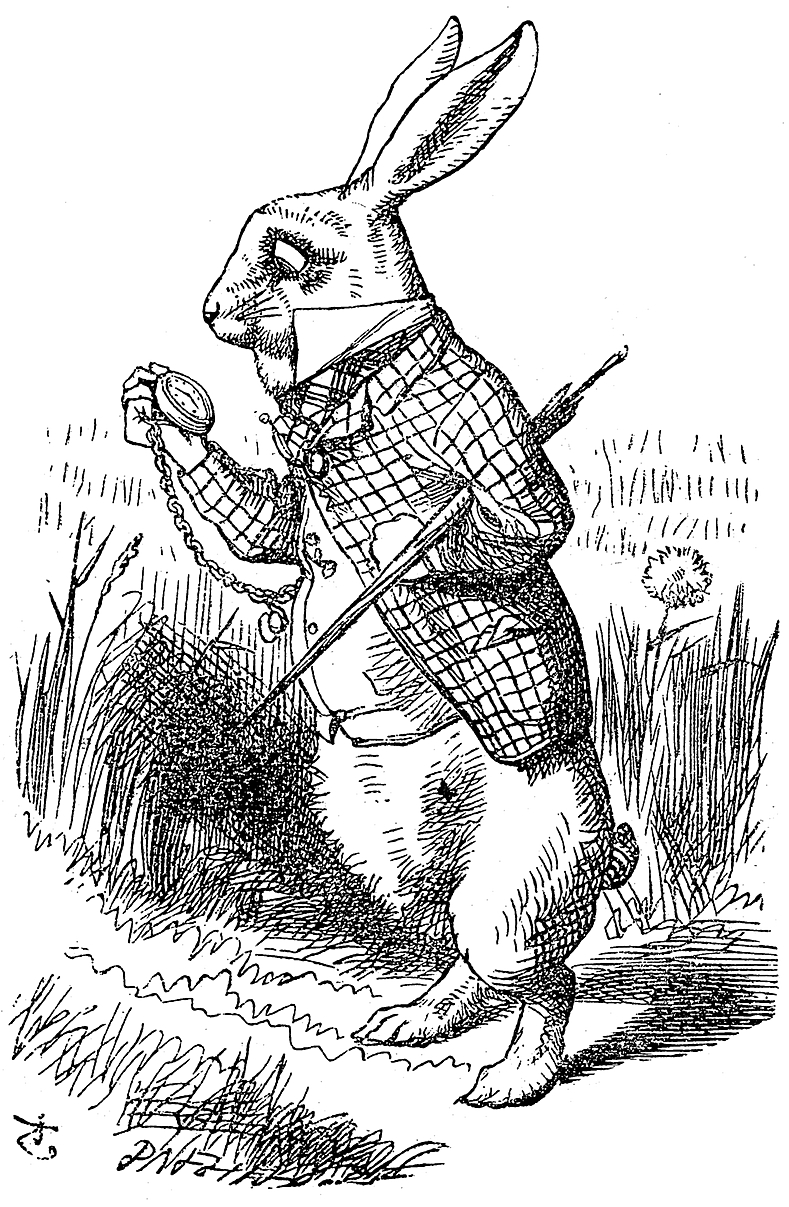
\includegraphics[height=5cm]{misc/Alice-wr.jpg}
\end{center}
\begin{center}
\textit{Oh dear! Oh dear! I shall be too late!}\\
\begin{small}
The White Rabbit in charge of real time
\end{small}
\end{center}
\end{frame}
%%%%%%%%%%%%%%%%%%%%%%%%%%%%%%%%%%%%%%%%%%%%%%%%%%%%%%%%%%%%%%%%%%%%%%%%%%%%%%%%%%%%%%%%%%%%%%%%%%%%

\begin{frame}{What is White Rabbit?}

\begin{columns}[c]
	\column{0.8\textwidth}
	  \begin{itemize}
		\item Renovation of accelerator's control and timing
		\item Based on well-known technologies
		\item Open Hardware and Open Software with commercial support
		\item International collaboration
    \item Many users: CERN, GSI, KM3NET, cosmic ray detectors, metrology labs...
	  \end{itemize}
	\column{0.3\textwidth}
		\begin{center}
		
\includegraphics[width=1.0\textwidth]{logo/WRlogo.pdf}
		\end{center}
	\end{columns}
\end{frame}
%%%%%%%%%%%%%%%%%%%%%%%%%%%%%%%%%%%%%%%%%%%%%%%%%%%%%%%%%%%%%%%%%%%%%%%%%%%%%%%%%%%%%%%%%%%%%%%%%%%%

\begin{frame}{Why we use Open Hardware ?}
  \begin{center}
    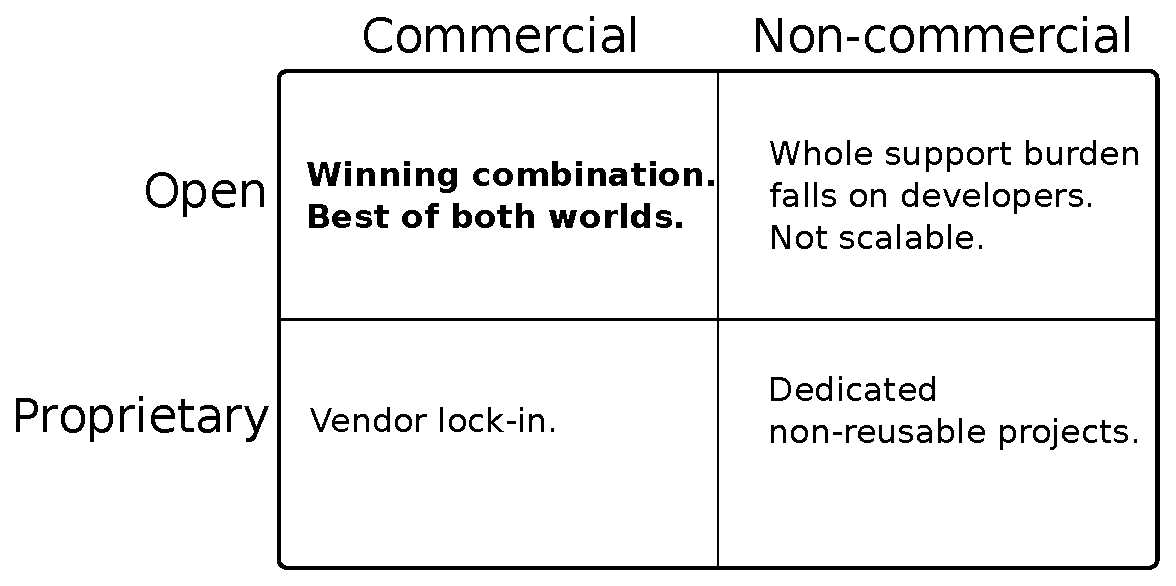
\includegraphics[width=.7\textwidth]{ohwr/commercial_and_open.pdf}
  \end{center}
  \begin{itemize}
    \item Get a design just the way we want it
    \item Peer review
    \item Healthier relationship with companies
  \end{itemize}
\end{frame}
%%%%%%%%%%%%%%%%%%%%%%%%%%%%%%%%%%%%%%%%%%%%%%%%%%%%%%%%%%%%%%%%%%%%%%%%%%%%%%%%%%%%%%%%%%%%%%%%%%%%
\begin{frame}{White Rabbit features}

\begin{columns}[c]
	\column{0.5\textwidth}
	  \begin{itemize}
		  \item Ethernet-based
        \begin{itemize}
		      \item thousands-nodes system
		      \item tens-km span
        \end{itemize}
      \item Synchronism
        \begin{itemize}
		      \item sub-ns accuracy
		      \item tens-ps precision
        \end{itemize}
      \item Determinism
        \begin{itemize}
		      \item upper-bound low-latency
		      \item high reliability
        \end{itemize}
	  \end{itemize}
	\column{0.5\textwidth}
		\begin{center}
		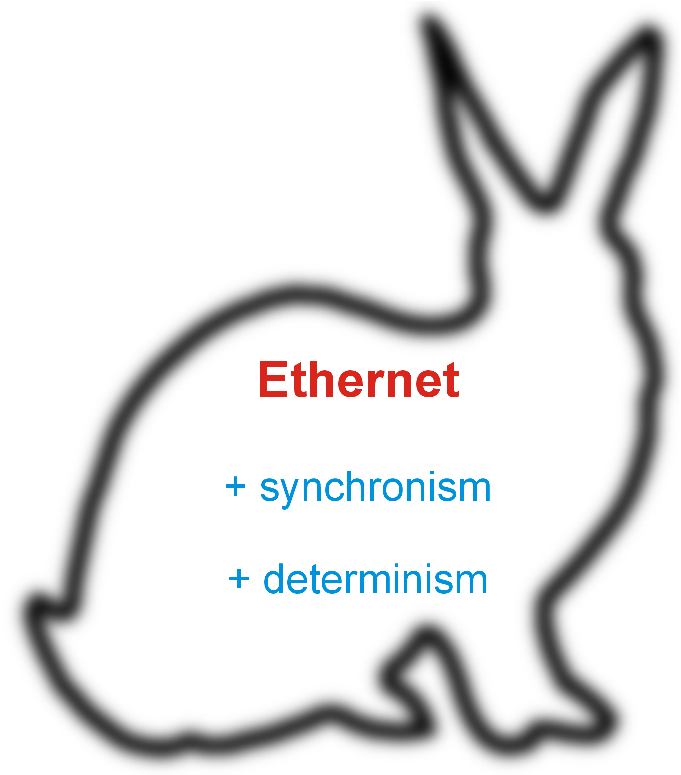
\includegraphics[width=1.0\textwidth]{misc/rabbit.pdf}
		\end{center}
	\end{columns}

\end{frame}
%%%%%%%%%%%%%%%%%%%%%%%%%%%%%%%%%%%%%%%%%%%%%%%%%%%%%%%%%%%%%%%%%%%%%%%%%%%%%%%%%%%%%%%%%%%%%%%%%%%%

\section[WR Network]{White Rabbit Network}
\subsection{}
\begin{frame}<beamer>{Outline}
    \tableofcontents [currentsection]
\end{frame}

%%%%%%%%%%%%%%%%%%%%%%%%%%%%%%%%%%%%%%%%%%%%%%%%%%%%%%%%%%%%%%%%%%%%%%%%%%%%%%%%%%%%%%%%%%%%%%%%%%%%
\begin{frame}{White Rabbit Network}


\begin{columns}[c]
  \column{.5\textwidth}
 
  \begin{itemize}
      \item Standard Ethernet network
      \item Ethernet features (VLAN) \& protocols (SNMP)
    \end{itemize}
    \begin{itemize}
      \item \color{Blue}{High accuracy synchronization}
      \item \color{Red}{Reliable and low-latency Control Data}
  \end{itemize}

  \column{.6\textwidth}
    \begin{center}
    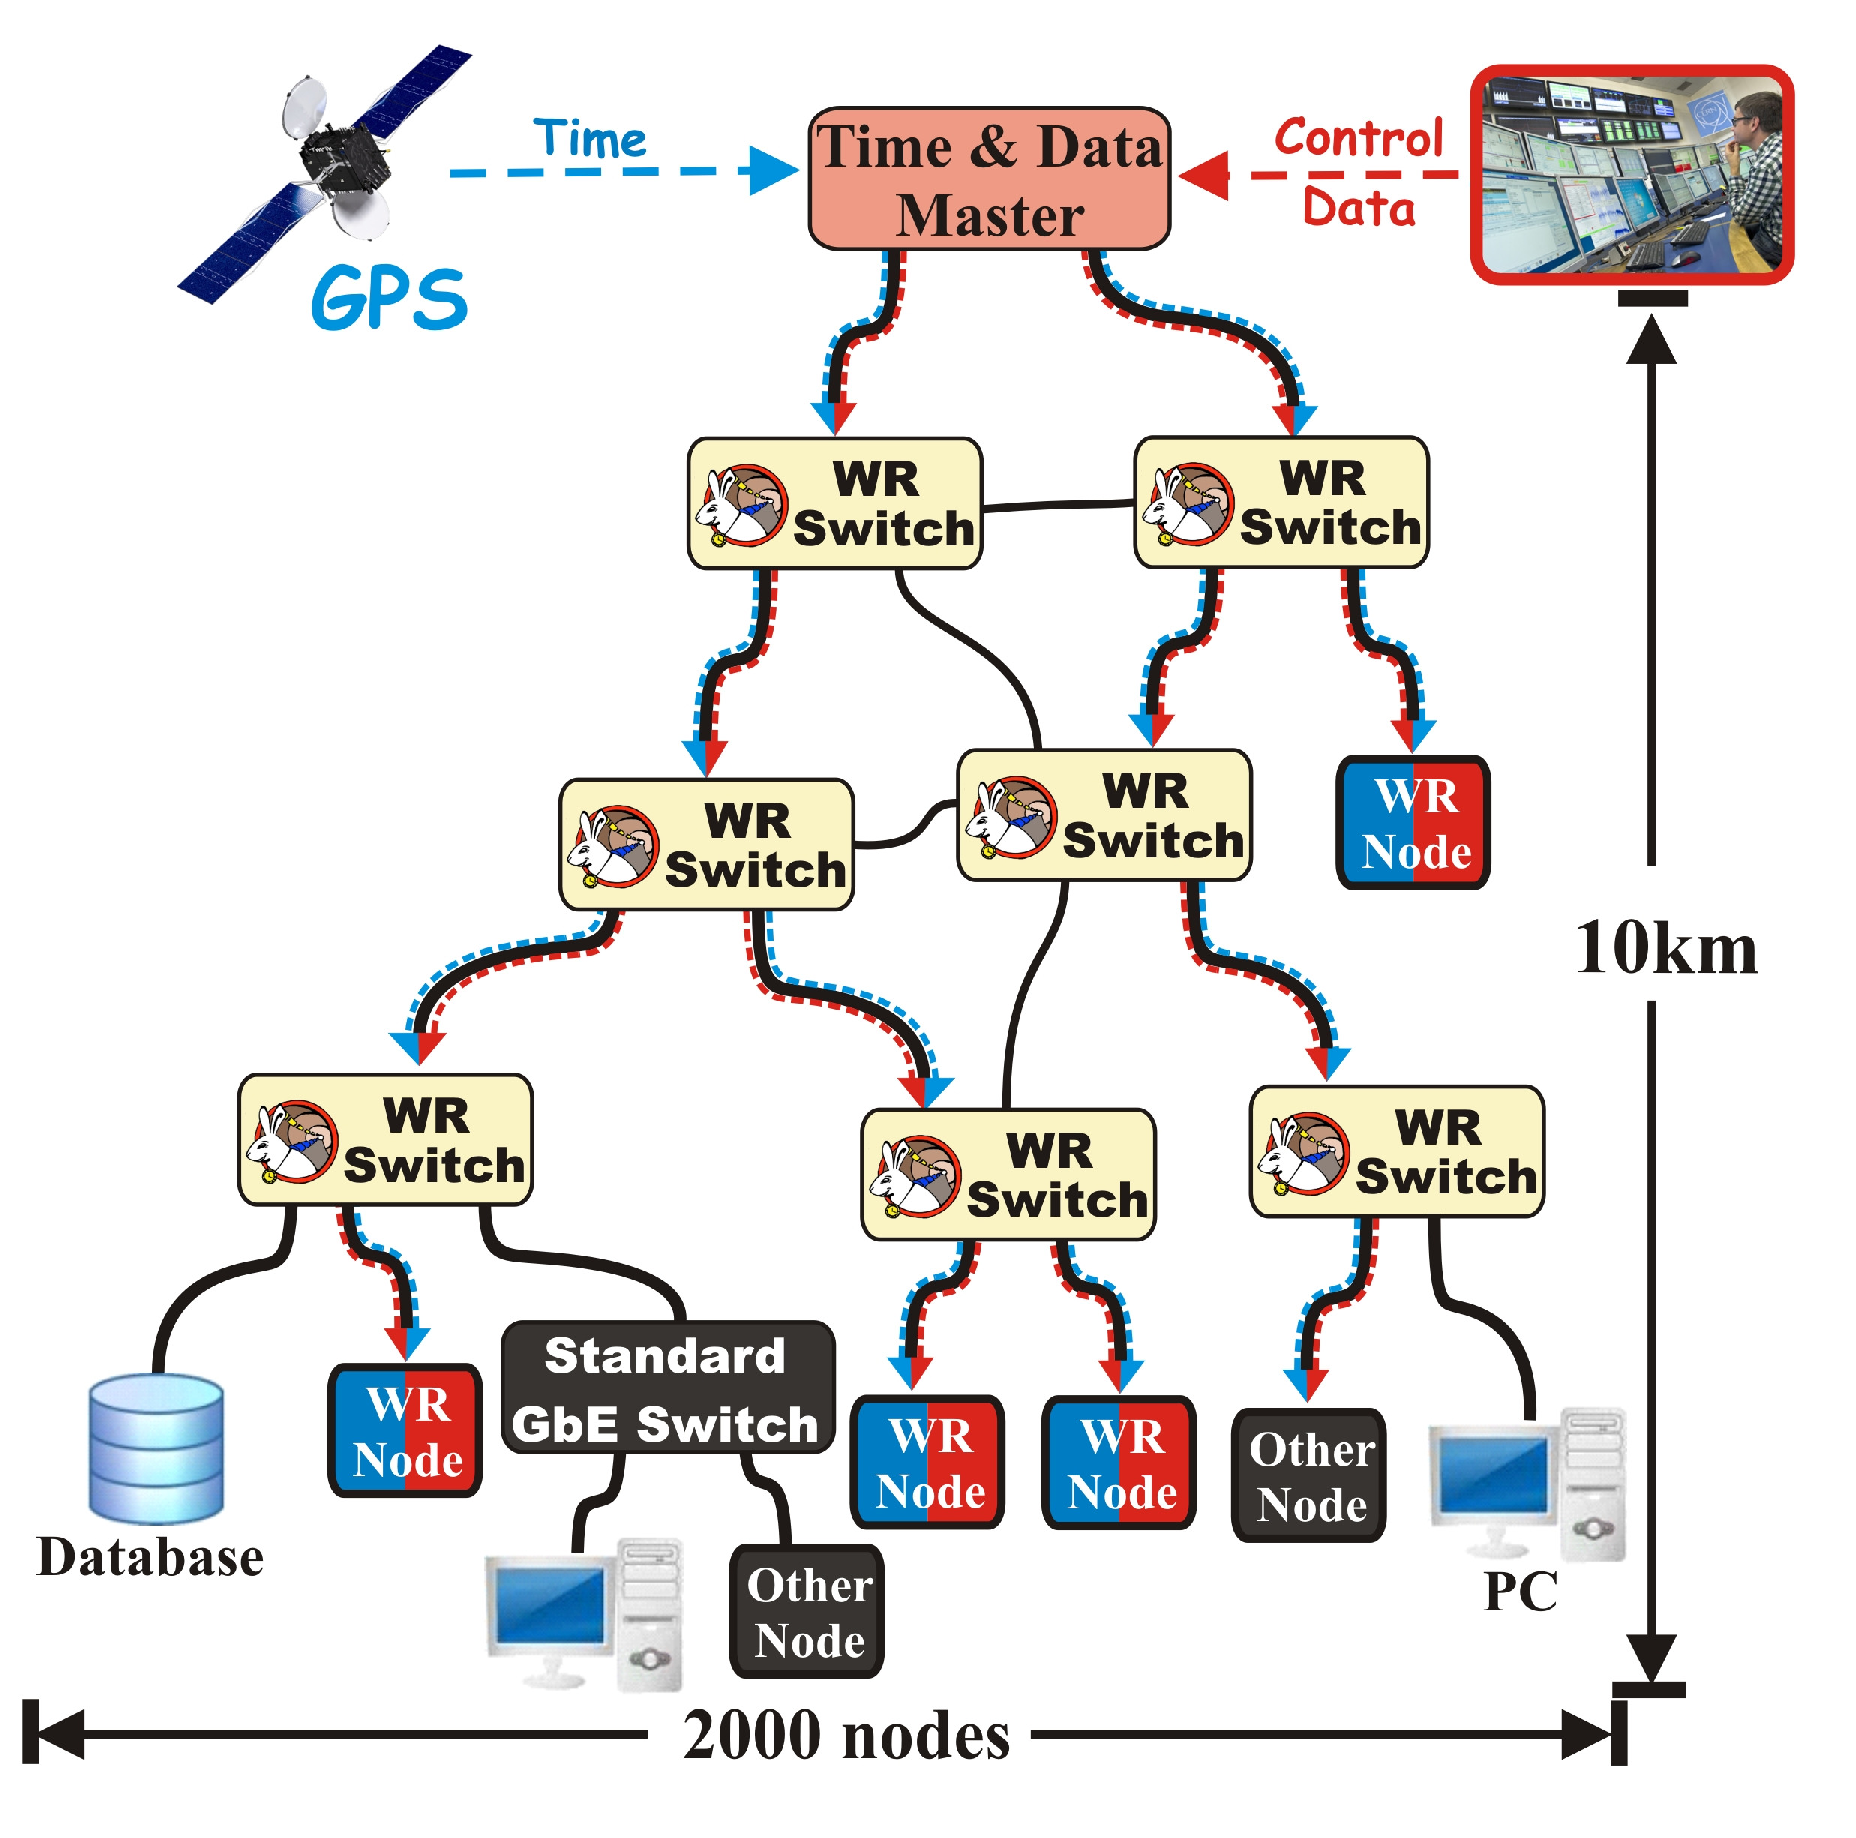
\includegraphics[height=1.05\textwidth]{network/wr_network-enhanced_pro.pdf}
    \end{center}
\end{columns}

\end{frame}

%%%%%%%%%%%%%%%%%%%%%%%%%%%%%%%%%%%%%%%%%%%%%%%%%%%%%%%%%%%%%%%%%%%%%%%%%%%%%%%%%%%%%%%%%%%%%%%%%%%%
\begin{frame}{White Rabbit Switch }

    \begin{center}
    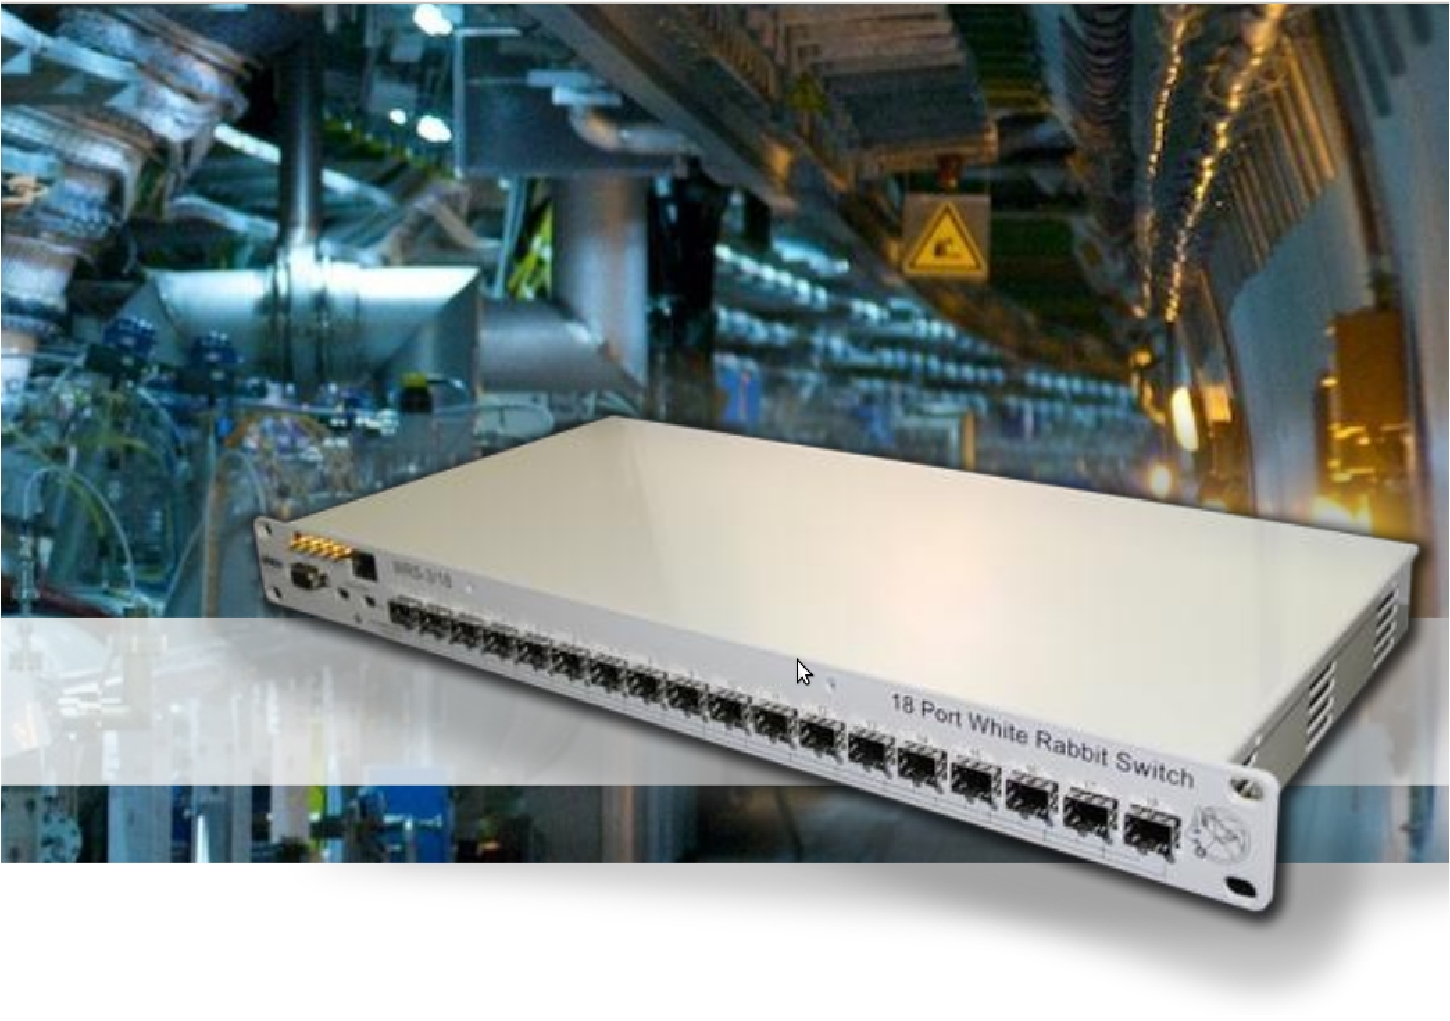
\includegraphics[width=6.0cm]{switch/wrSwitchV3.jpg}
    \end{center}

	\begin{itemize}
	\item Central element of WR network
	\item Designed from scratch
	\item 18 ports
	\item 1000BASE-BX10 SFPs: up to 10 km, single-mode fiber
	\item Open design (H/W and S/W)
	\end{itemize}
\end{frame}

%%%%%%%%%%%%%%%%%%%%%%%%%%%%%%%%%%%%%%%%%%%%%%%%%%%%%%%%%%%%%%%%%%%%%%%%%%%%%%%%%%%%%%%%%%%%%%%%%%%%
\begin{frame}{White Rabbit Node}
  Modular hardware kit:
  \begin{itemize}
    \item set of Mezzanine boards: ADC, DAC, TDC, Fine delay...
    \item set of carriers for various needs: PCIe, VME64x, PXIe...
    \item all carriers equipped with a White Rabbit port
  \end{itemize}
  \begin{center}
  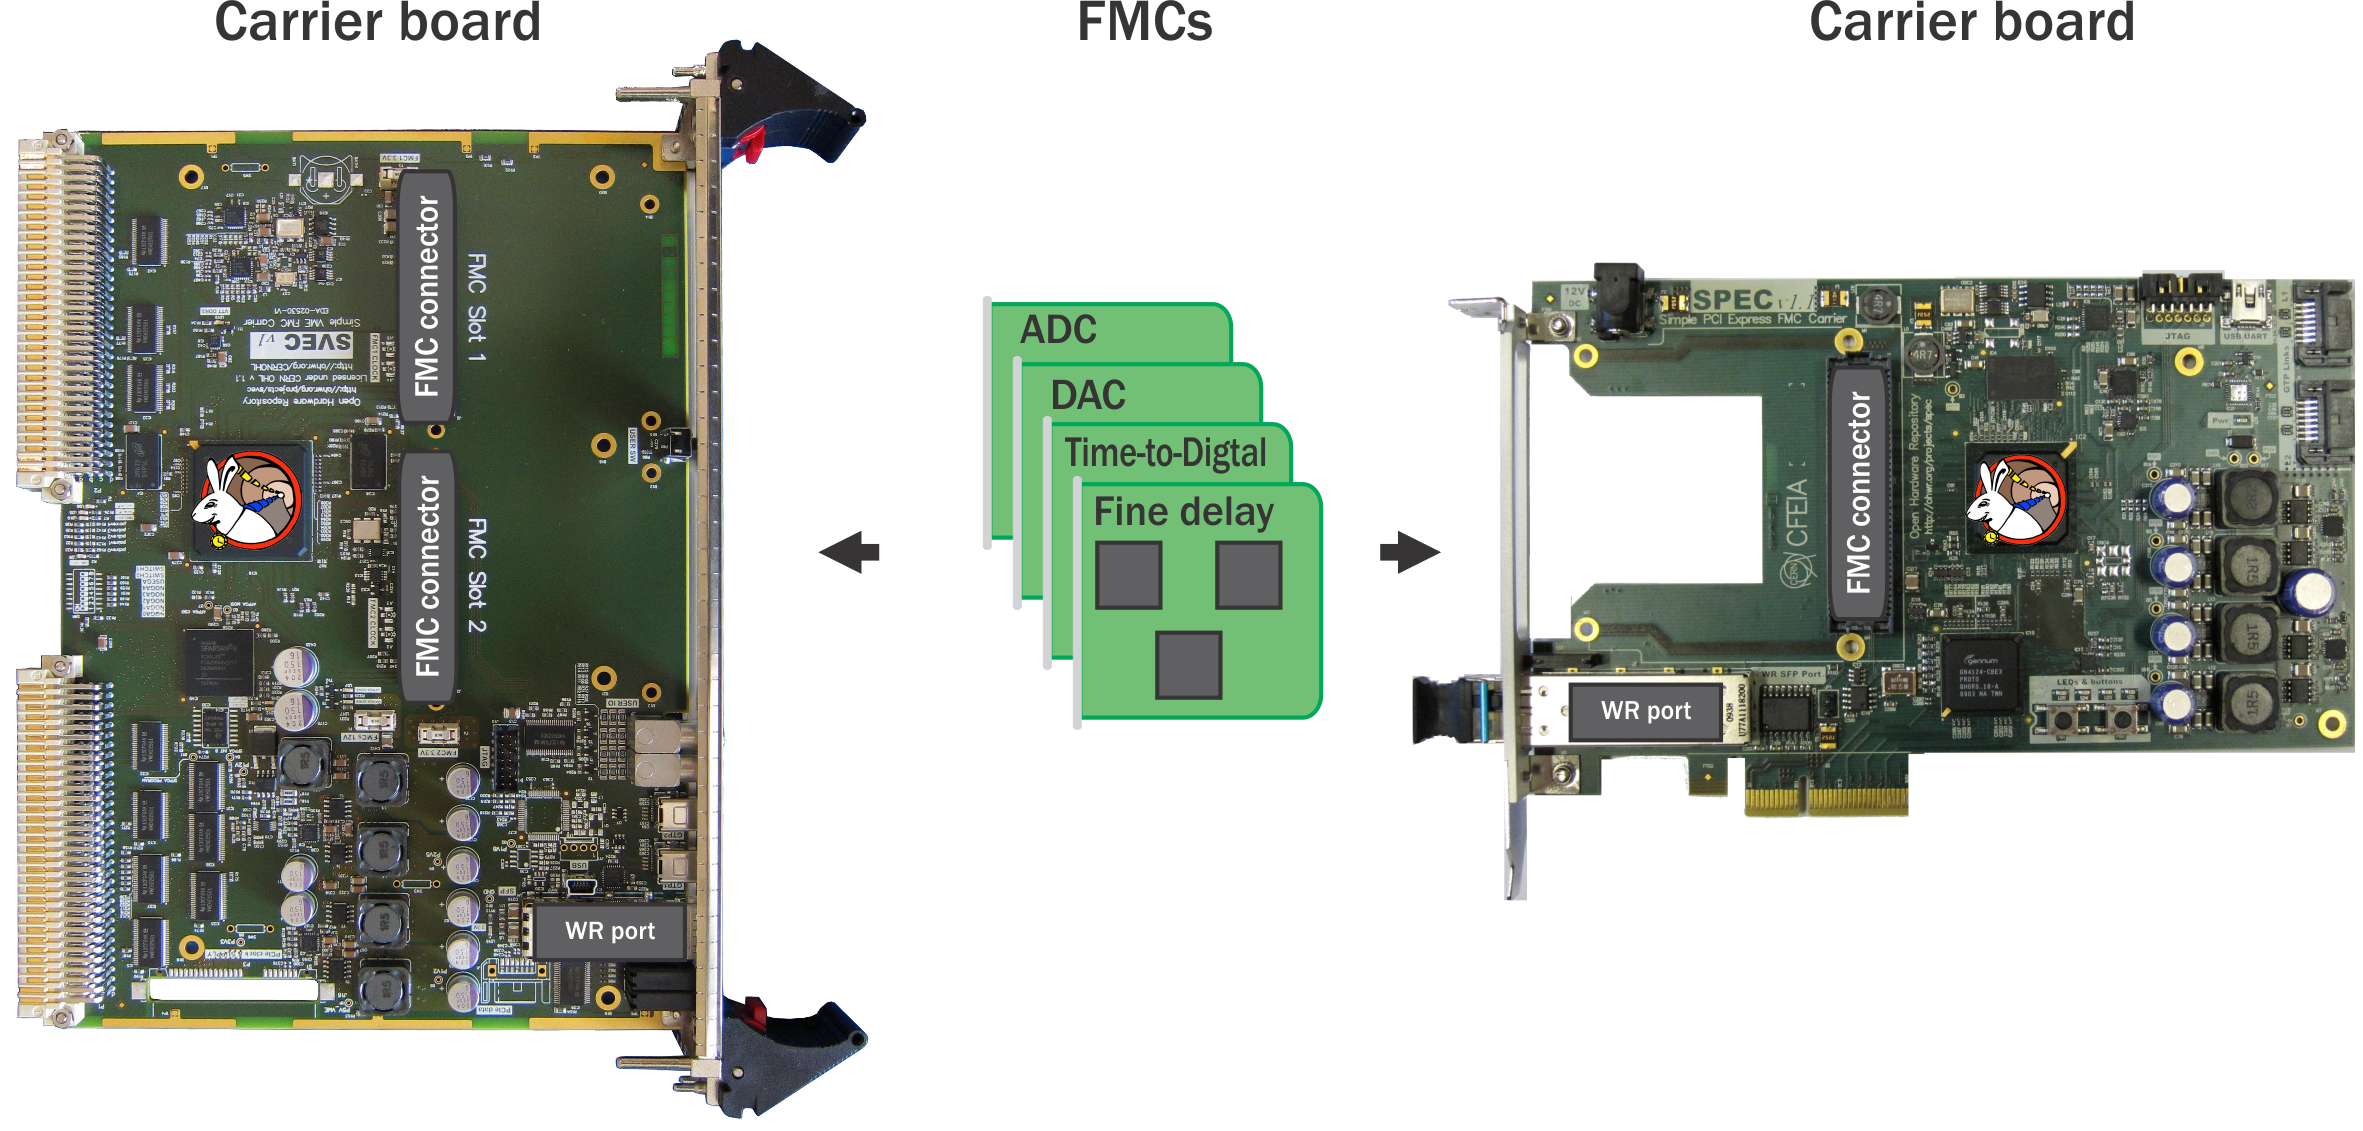
\includegraphics[height=0.5\textheight]{node/shw_kit2.png}
  \end{center}
\end{frame}

\begin{frame}{White Rabbit Node - example}
  \begin{center}
  \includegraphics<1>[width=\textwidth]{node/specInterior2.pdf}
  \includegraphics<2>[width=\textwidth]{network/kit_sync1.png}
  \includegraphics<3>[width=\textwidth]{network/kit_sync2.png}
  \includegraphics<4>[width=\textwidth]{network/kit_sync3.png}
  \includegraphics<5>[width=\textwidth]{network/kit_sync4.png}
  \end{center}
\end{frame}

\begin{frame}{White Rabbit PTP Core}

	\begin{itemize}
	  \item Fancy Ethernet MAC with White Rabbit support
	  \item Open IP Core
	  \item Easily integrated into custom FPGA-based designs
	\end{itemize}

    \begin{center}
    \includegraphics<1>[height=0.5\textheight]{node/wrpc_overview.pdf}
    \end{center}
\end{frame}

\begin{frame}{Open Hardware Repository (OHWR)}
  \begin{columns}
    \column{.7\textwidth}
    \begin{itemize}
      \item All schematics, HDL designs and software sources available in OHWR
      \item Over 100 projects currently hosted
      \item 11 scientific institutes and 16 companies involved
    \end{itemize}
    \column{.4\textwidth}
    \begin{center}
      
\includegraphics[width=\textwidth]{ohwr/ohr_logo.pdf}
      \begin{block}{}
        \begin{center}
        \url{http://www.ohwr.org}
        \end{center}
      \end{block}
    \end{center}
  \end{columns}
\end{frame}


%%%%%%%%%%%%%%%%%%%%%%%%%%%%%%%%%%%%%%%%%%%%%%%%%%%%%%%%%%%%%%%%%%%%%%%%%%%%%%%%%%%%%%%%%%%%%%%%%%%%
\section{Time Distribution~~~}
\subsection{}
%%%%%%%%%%%%%%%%%%%%%%%%%%%%%%%%%%%%%%%%%%%%%%%%%%%%%%%%%%%%%%%%%%%%%%%%%%%%%%%%%%%%%%%%%%%%%%%%%%%%
\begin{frame}<beamer>{Outline}
    \tableofcontents [currentsection]
\end{frame}
%%%%%%%%%%%%%%%%%%%%%%%%%%%%%%%%%%%%%%%%%%%%%%%%%%%%%%%%%%%%%%%%%%%%%%%%%%%%%%%%%%%%%%%%%%%%%%%%%%%%
\begin{frame}{Time Distribution in White Rabbit Network}

  \begin{itemize}
    \item Synchronization with {\bf sub-ns} accuracy {\bf tens-ps} precision
    \item Combination of
	\begin{itemize}
	  \item Precision Time Protocol  ({\bf IEEE1588})  synchronization
	  \item Layer 1 syntonization
	  \item Phase measurements
	\end{itemize}
  \end{itemize}
\end{frame}

%%%%%%%%%%%%%%%%%%%%%%%%%%%%%%%%%%%%%%%%%%%%%%%%%%%%%%%%%%%%%%%%%%%%%%%%%%%%%%%%%%%%%%%%%%%%%%%%%%%%
\begin{frame}{Precision Time Protocol (IEEE1588)}

\begin{columns}[c]
  \column{1.2in}
  \begin{center}
    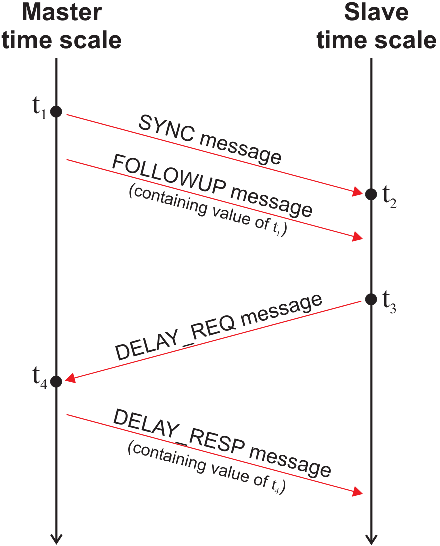
\includegraphics[height=5cm]{protocol/ptp_exchange.pdf}
  \end{center}
  \column{3in}
    
  
  \begin{itemize}
    \item Simple calculations:
    \begin{itemize}
      \item link $delay_{ms}$: $\delta_{ms} = \frac{(t_{4}-t_{1}) - (t_{3}-t_{2})}{2}$
      \item clock $offset_{ms} = t_{2} - t_{1} + \delta_{ms}$
    \end{itemize}
   \item<2> Disadvantages
     \begin{itemize}
       \item assumes symmetry of medium
       \item all nodes have free-running oscillators
       \item frequency drift compensation vs. message exchange traffic
     \end{itemize}
   \end{itemize}
\end{columns}

\end{frame}

%%%%%%%%%%%%%%%%%%%%%%%%%%%%%%%%%%%%%%%%%%%%%%%%%%%%%%%%%%%%%%%%%%%%%%%%%%%%%%%%%%%%%%%%%%%%%%%%%%%%
\begin{frame}{Layer 1 Syntonization}

  \begin{center}
    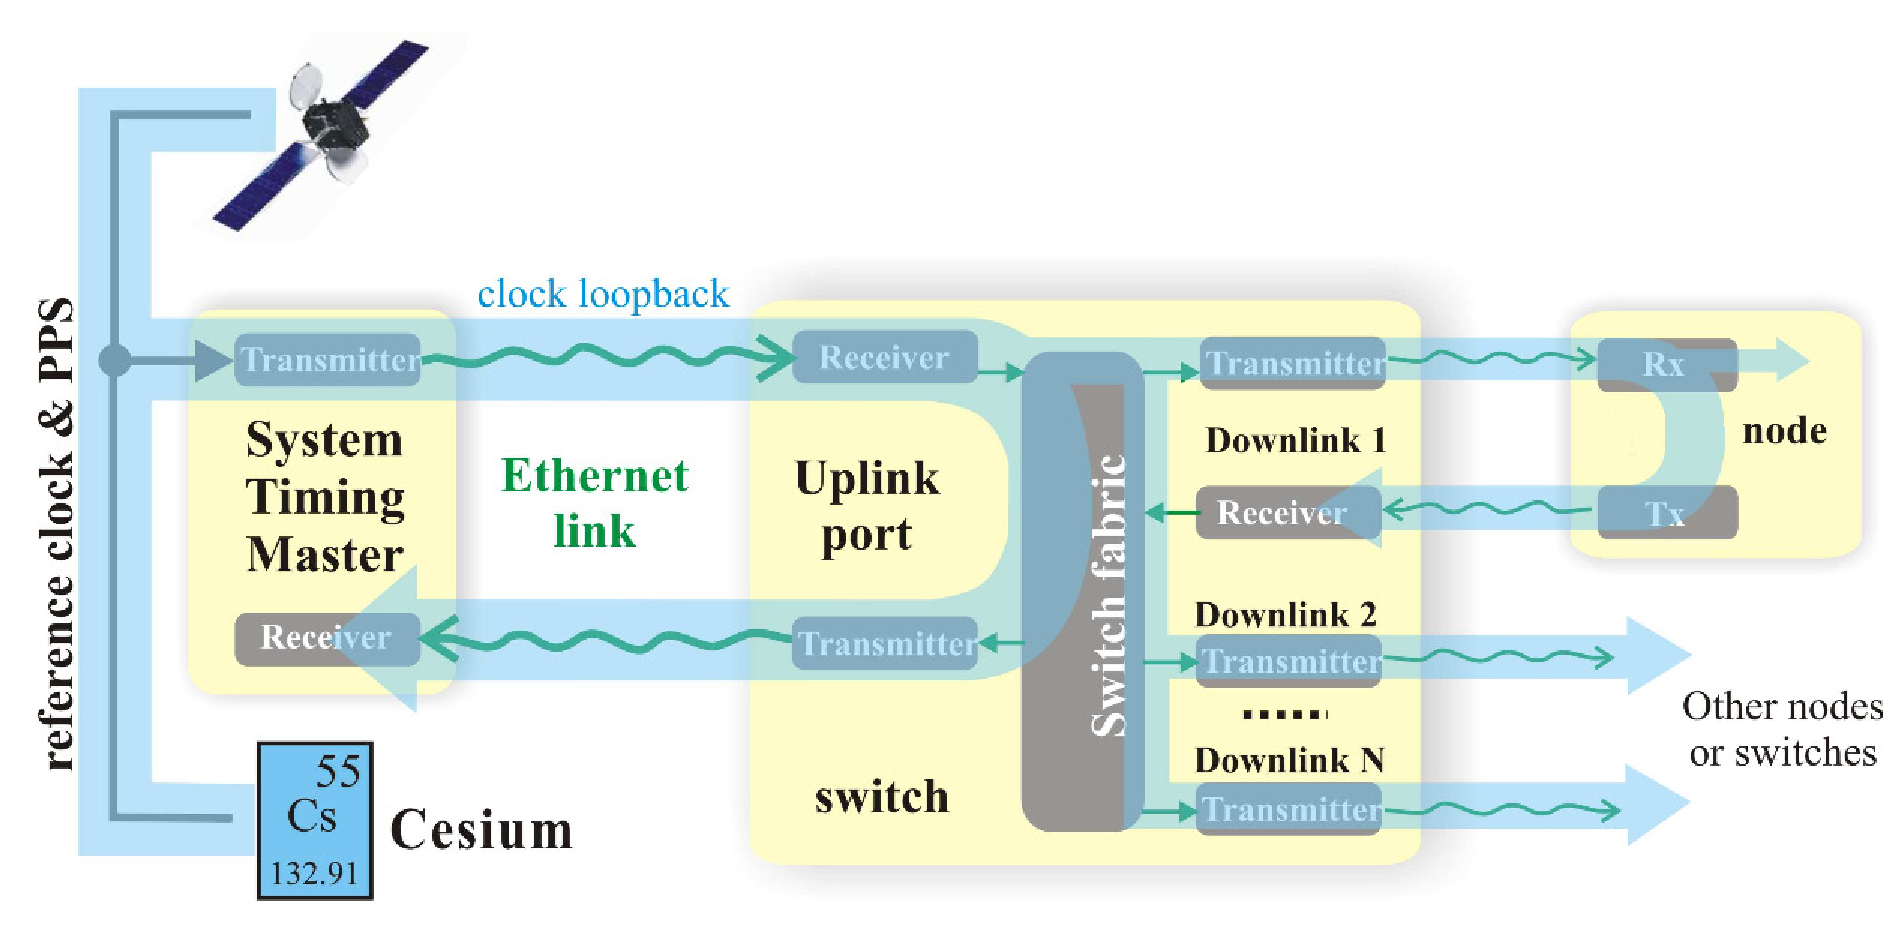
\includegraphics[width=1.0\textwidth]{misc/l1_sync.pdf}
  \end{center}
\end{frame}

%%%%%%%%%%%%%%%%%%%%%%%%%%%%%%%%%%%%%%%%%%%%%%%%%%%%%%%%%%%%%%%%%%%%%%%%%%%%%%%%%%%%%%%%%%%%%%%%%%%%
\begin{frame}{Phase measurements}

  \begin{itemize}
    \item Monitor phase of bounced-back clock
    \item Enhance PTP timestamps with phase measurement
    \item Phase-locked loop in the slave follows the phase changes  
  \end{itemize}

  \begin{center}
    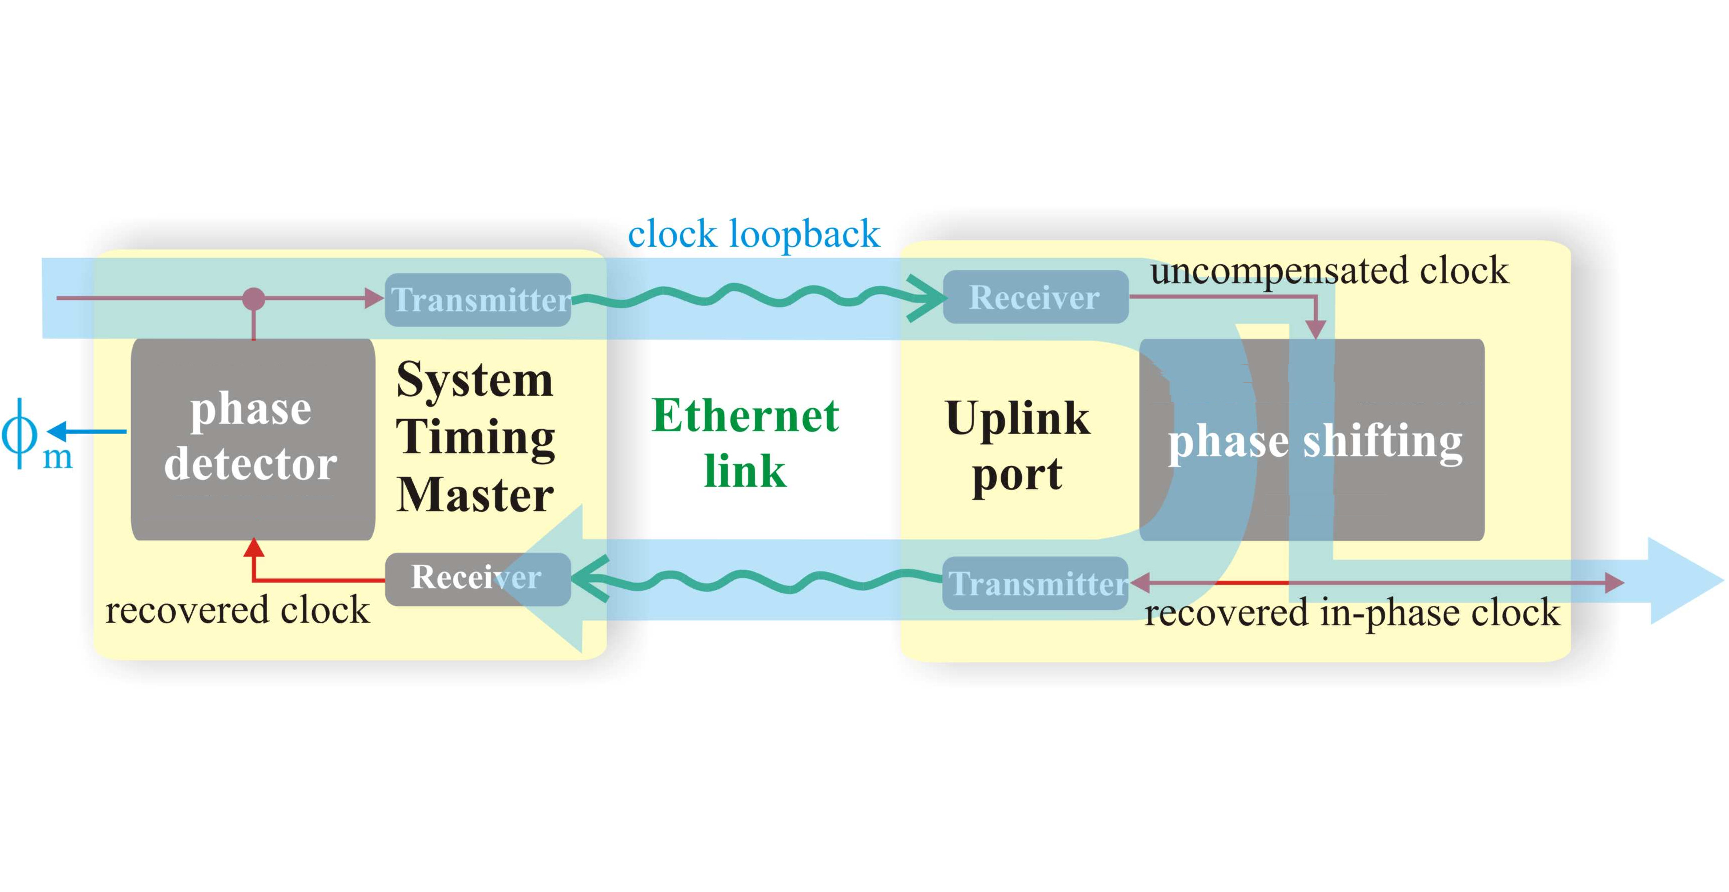
\includegraphics[width=1.0\textwidth]{misc/phase_tracking_v2_simple.pdf}
  \end{center}

\end{frame}

%%%%%%%%%%%%%%%%%%%%%%%%%%%%%%%%%%%%%%%%%%%%%%%%%%%%%%%%%%%%%%%%%%%%%%%%%%%%%%%%%%%%%%%%%%%%%%%%%%%%
\begin{frame}{WR synchronization performance}

    \begin{center}
    \includegraphics<1>[height=7.0cm]{measurements/meas_setup.pdf}
    \includegraphics<2->[height=5.0cm]{measurements/meas_results.pdf}
    \onslide<3> {
    \begin{columns}[c]
      \column{.7\textwidth}
    \begin{block}{  \begin{center} ISPCS Plug Fest \end{center}}
      \begin{center}
	      \textbf{WR: most accurate PTP implementation in the world!}
      \end{center}
    \end{block}
    \end{columns}}
    \end{center}

\end{frame}

%%%%%%%%%%%%%%%%%%%%%%%%%%%%%%%%%%%%%%%%%%%%%%%%%%%%%%%%%%%%%%%%%%%%%%%%%%%%%%%%%%%%%%%%%%%%%%%%%%%%
\begin{frame}{WR Standardization under IEEE1588}

\begin{columns}[c]
  \column{0.5\textwidth}
    \begin{itemize}
      \item <1->We want to standardize!
      \item <2->Intention by 1588 Standardization Group expressed in Project
        Authorization Request
      \item <3->Enhanced Accuracy Options / Profile
    \end{itemize}
  \column{0.5\textwidth}

    \begin{center}
       \includegraphics<1>[width=1.0\textwidth]{misc/PTPv3_blank.pdf} 
       \includegraphics<2>[width=1.0\textwidth]{misc/PTPv3_PAR.pdf} 
       \includegraphics<3>[width=1.0\textwidth]{misc/PTPv3-wr-2.pdf}
    \end{center}

\end{columns}

\end{frame}

%%%%%%%%%%%%%%%%%%%%%%%%%%%%%%%%%%%%%%%%%%%%%%%%%%%%%%%%%%%%%%%%%%%%%%%%%%%%%%%%%%%%%%%%%%%%%%%%%%%%
\section{Data Distribution}
\subsection{}
%%%%%%%%%%%%%%%%%%%%%%%%%%%%%%%%%%%%%%%%%%%%%%%%%%%%%%%%%%%%%%%%%%%%%%%%%%%%%%%%%%%%%%%%%%%%%%%%%%%%
\begin{frame}<beamer>{Outline}
    \tableofcontents [currentsection]
\end{frame}

%%%%%%%%%%%%%%%%%%%%%%%%%%%%%%%%%%%%%%%%%%%%%%%%%%%%%%%%%%%%%%%%%%%%%%%%%%%%%%%%%%%%%%%%%%%%%%%%%%%%%
\begin{frame}{Data Distribution in a White Rabbit Network }

    \vspace{-0.3cm}

    \begin{center}
    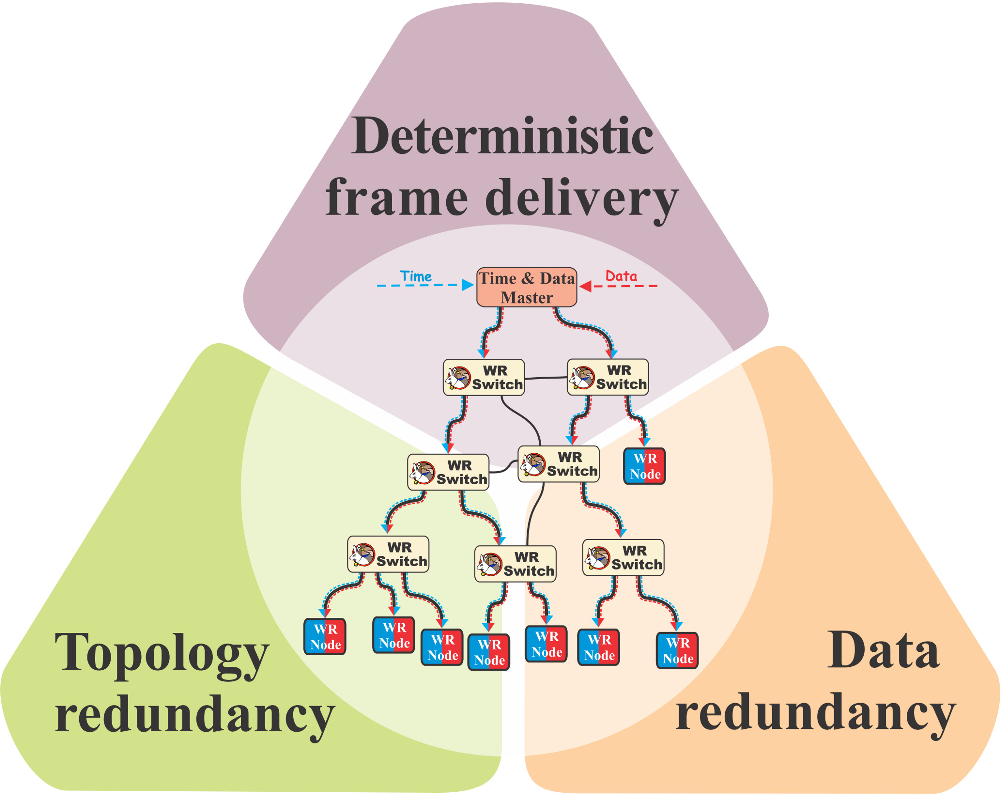
\includegraphics[height=0.8\textheight]{robustness/wrn_reliability.pdf}
    \end{center}
	  
    \vspace{-0.7cm}

\end{frame}

%%%%%%%%%%%%%%%%%%%%%%%%%%%%%%%%%%%%%%%%%%%%%%%%%%%%%%%%%%%%%%%%%%%%%%%%%%%%%%%%%%%%%%%%%%%%%%%%%%%%
\begin{frame}{Deterministic data delivery}

\begin{columns}[c]
  \column{.55\textwidth}
    \begin{itemize}
      \item Types of data distinguished by 802.1Q tag:
	  \begin{itemize}
	    \item \textcolor{red}{\bf Control Data} (strict priority)
	    \item Standard Data (Best Effort)
	  \end{itemize}
	  \item \textcolor{red}{\bf Control Data} characteristics:
	  \begin{itemize}
      \item Sent by Data Master(s)
	    \item Broadcast (one-to-many)
	    \item Deterministic and low-latency
	    \item Reliable delivery
	  \end{itemize}
    \item Low-latency WR Switch by design ( \textcolor{red}{$<10$us} )
    \end{itemize}
  \column{.6\textwidth}
    \begin{center}
    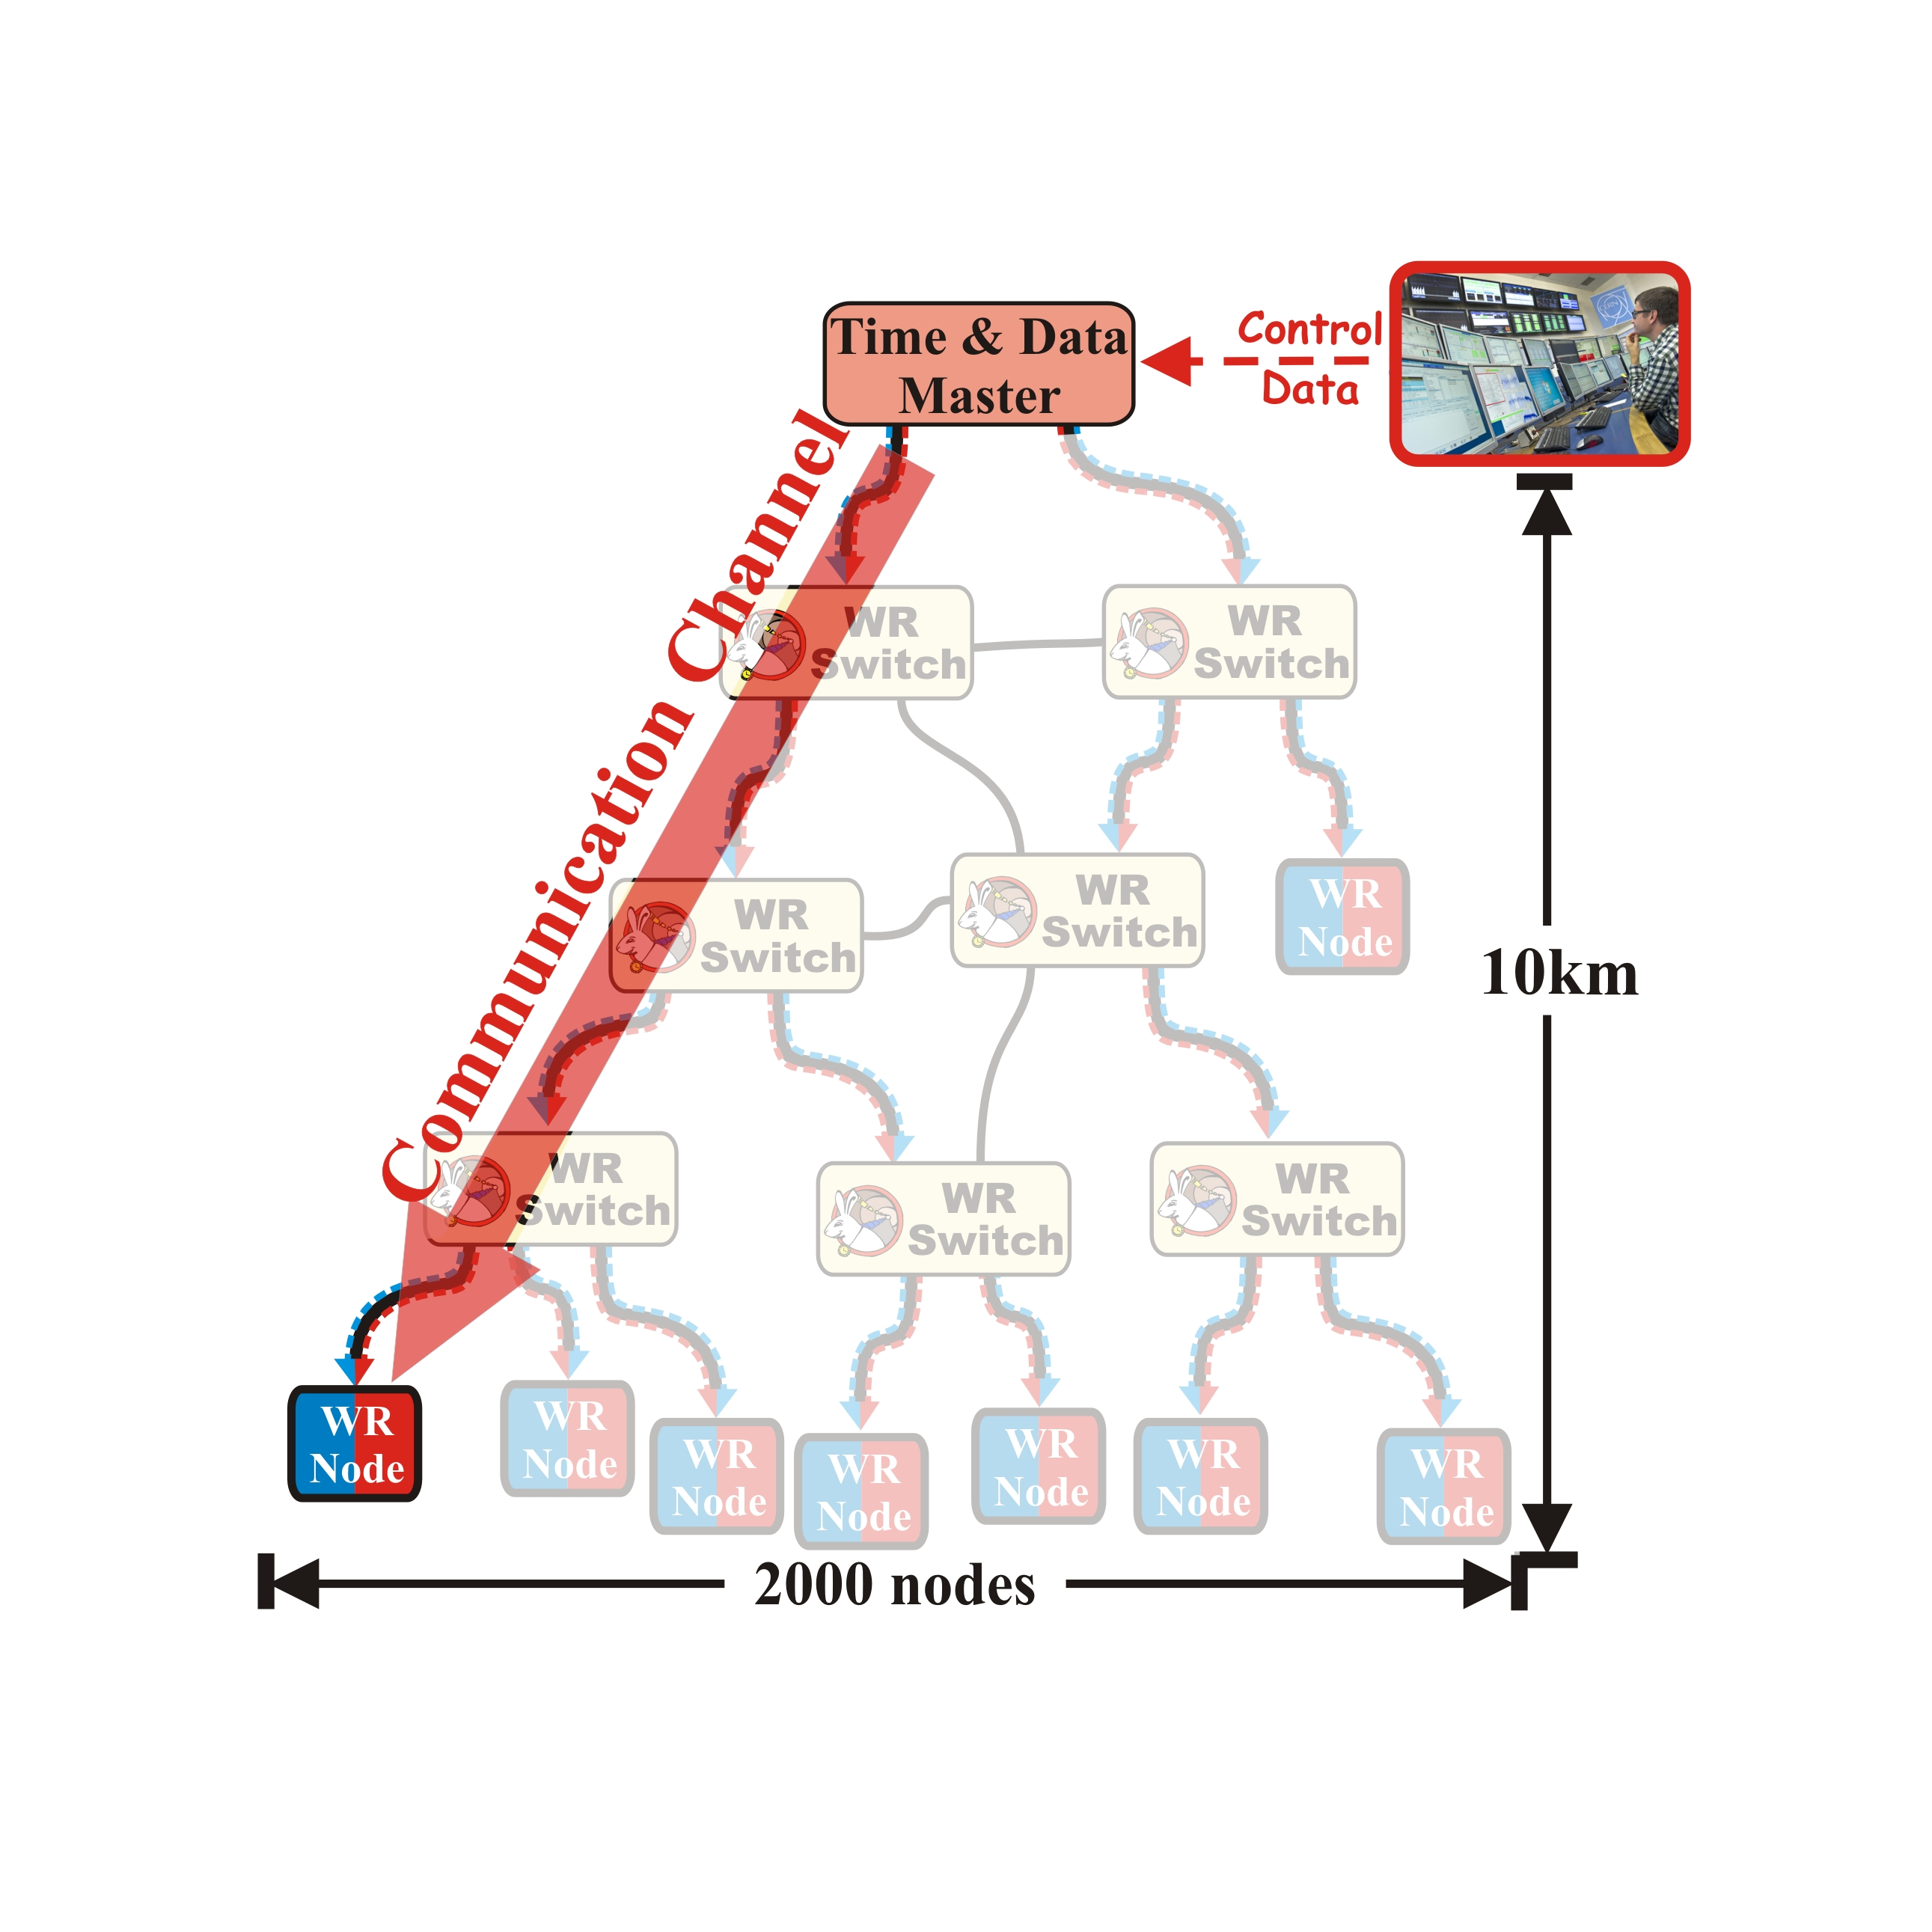
\includegraphics[height=0.65\textheight]{robustness/communication_channel-pro.jpg}
    \end{center}

\end{columns}
\end{frame}

%%%%%%%%%%%%%%%%%%%%%%%%%%%%%%%%%%%%%%%%%%%%%%%%%%%%%%%%%%%%%%%%%%%%%%%%%%%%%%%%%%%%%%%%%%%%%%%%%%%%
\begin{frame}{Data Redundancy (Node)}
   
  \begin{itemize}
	\item {\bf Forward Error Correction (FEC)}  -- transparent layer:
	\begin{itemize}
		\item One message encoded into 4 Ethernet frames
		\item Recovery of message from any 2 frames
	\end{itemize}
	\item <2->FEC can prevent data loss due to:
	\begin{itemize}	
		\item<3-> {\bf bit errors} 
		\item<4> {\bf network reconfiguration}
	\end{itemize}	
  \end{itemize}
  
  	\begin{center}
      
\includegraphics[width=.7\textwidth]{robustness/FEC.pdf}
    \end{center}
  
\end{frame}

%%%%%%%%%%%%%%%%%%%%%%%%%%%%%%%%%%%%%%%%%%%%%%%%%%%%%%%%%%%%%%%%%%%%%%%%%%%%%%%%%%%%%%%%%%%%%%%%%%%%
\begin{frame}{Topology Redundancy (Switch)}

  \begin{itemize}
	\item Ideas:
	\begin{itemize}
        \item Using VLANs
        \item H/W switch-over to the backup link
	      \item WR Rapid Spanning Tree Protocol
	      \item WR Shortest Path Bridging
	\end{itemize}
	\item Seamless redundancy requires Forward Error Correction
  \end{itemize}
  
\end{frame}

%%%%%%%%%%%%%%%%%%%%%%%%%%%%%%%%%%%%%%%%%%%%%%%%%%%%%%%%%%%%%%%%%%%%%%%%%%%%%%%%%%%%%%%%%%%%%%%%%%%%
\subsection{}
%%%%%%%%%%%%%%%%%%%%%%%%%%%%%%%%%%%%%%%%%%%%%%%%%%%%%%%%%%%%%%%%%%%%%%%%%%%%%%%%%%%%%%%%%%%%%%%%%%%%

\begin{frame}{Topology reconfiguration performance}

\begin{columns}[c]
  \column{0.45\textwidth}

    \begin{center}
    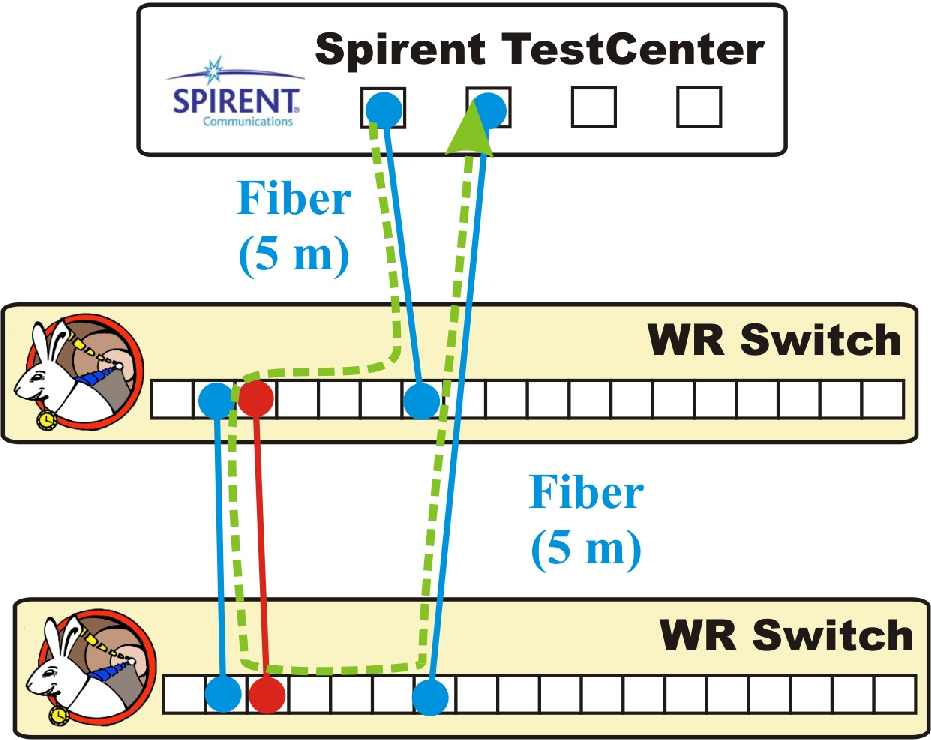
\includegraphics[width=1.0\textwidth]{robustness/switchover.pdf} 
    \end{center}

  \column{0.6\textwidth}
    \begin{center}
    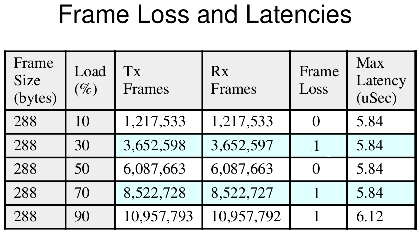
\includegraphics[width=1.0\textwidth]{robustness/switchover288-ok.pdf}
    \end{center}

\end{columns}
\end{frame}

%%%%%%%%%%%%%%%%%%%%%%%%%%%%%%%%%%%%%%%%%%%%%%%%%%%%%%%%%%%%%%%%%%%%%%%%%%%%%%%%%%%%%%%%%%%%%%%%%%%
\section{Applications}
\subsection{}
%%%%%%%%%%%%%%%%%%%%%%%%%%%%%%%%%%%%%%%%%%%%%%%%%%%%%%%%%%%%%%%%%%%%%%%%%%%%%%%%%%%%%%%%%%%%%%%%%%%%
\begin{frame}<beamer>{Outline}
    \tableofcontents [currentsection]
\end{frame}

\begin{frame}{Distributed oscilloscope}
  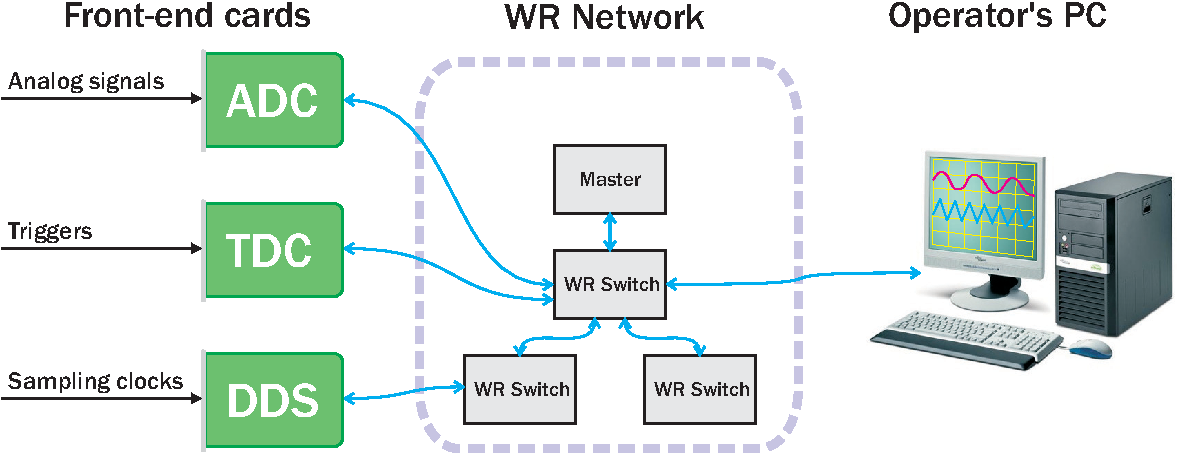
\includegraphics[width=.8\textwidth]{applications/distr_oscill.pdf}
  \begin{block}{}
    \begin{itemize}
      \item Common clock in the entire network: no skew between ADCs.
      \item Ability to sample with different clocks
      \item Internal time triggers or external asynchronous triggers time tagged
        with a TDC
    \end{itemize}
  \end{block}
\end{frame}

\begin{frame}{CERN Neutrinos to Gran Sasso project}
  \begin{center}
    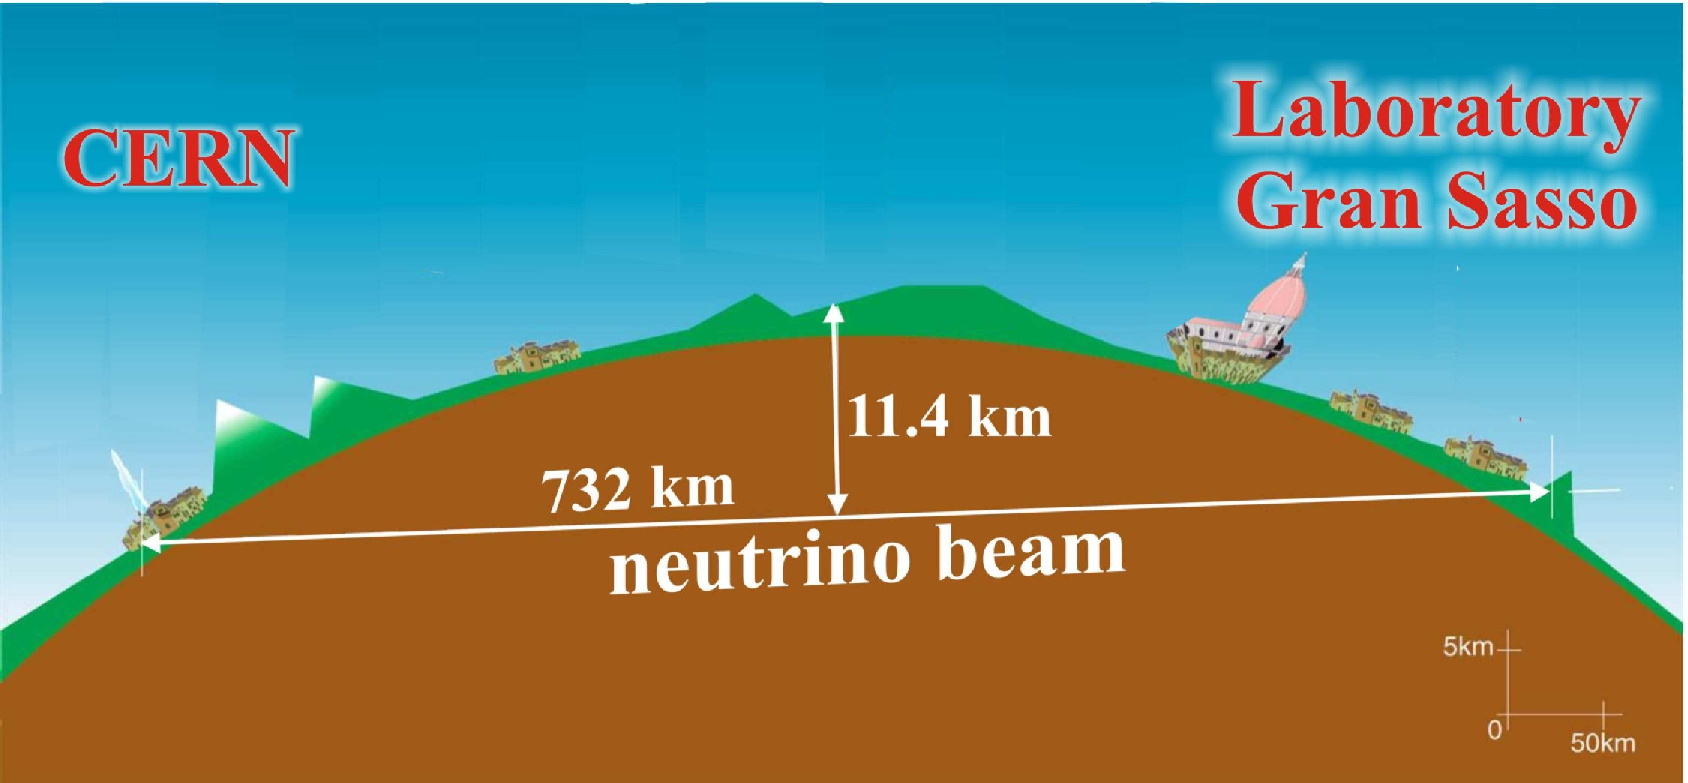
\includegraphics[width=.8\textwidth]{applications/cngs-general.pdf}
  \end{center}
  \begin{itemize}
    \item Investigation of neutrino oscillation
    \item Time of Flight measurement
  \end{itemize}
\end{frame}

\begin{frame}{CERN Neutrinos to Gran Sasso project}
  \only<1> {
    \begin{center}
      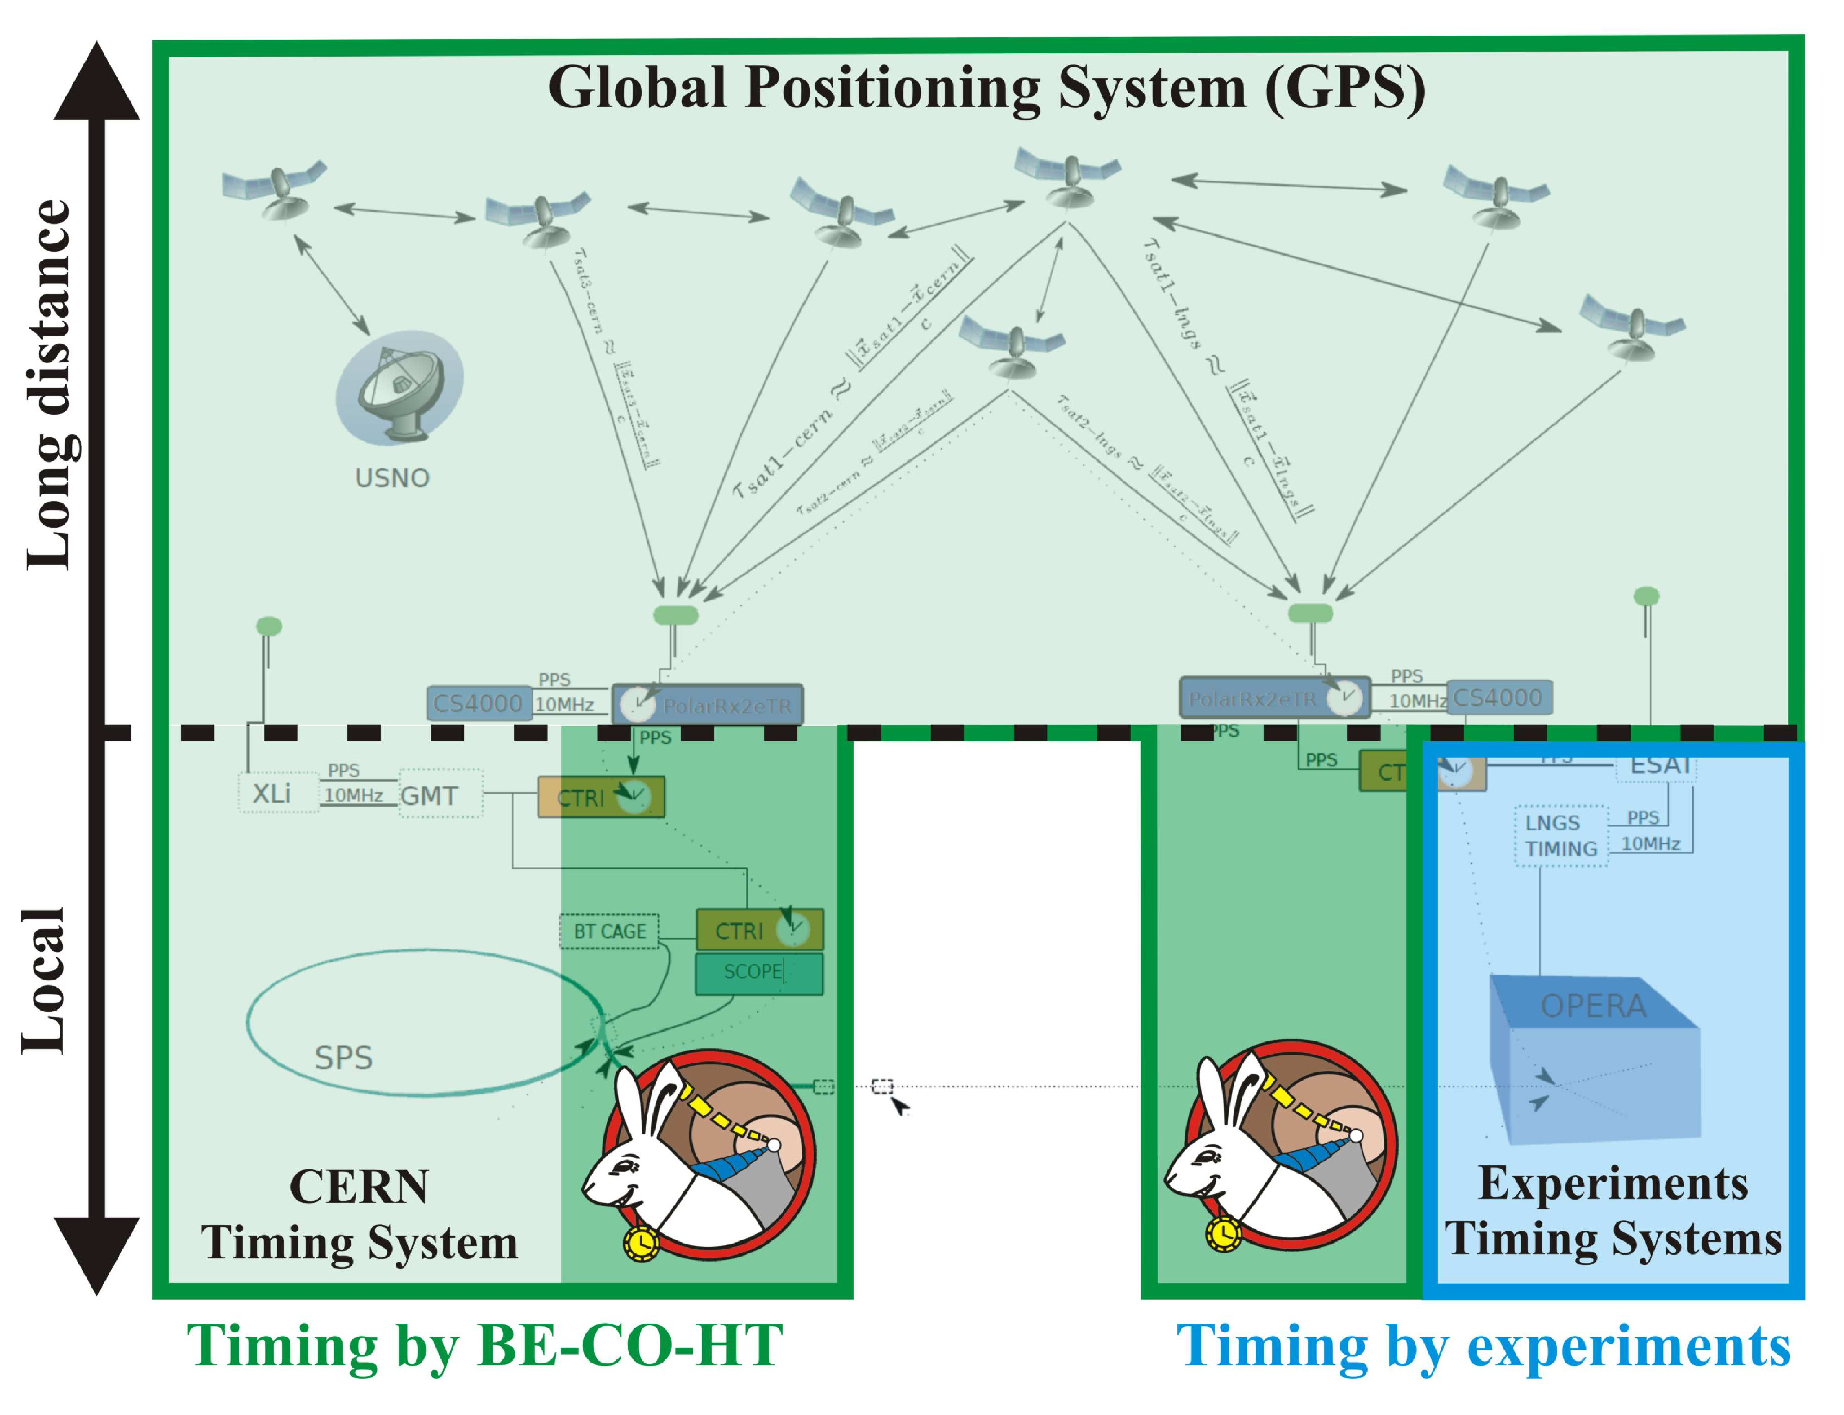
\includegraphics[width=.9\textwidth]{applications/cngs-timing-31.pdf}
    \end{center}
  }
 
  \only<2> {
  \begin{columns}[c]
    \column{.6\textwidth}
    \begin{itemize}
      \item WR transferring UTC from GPS receiver to the measurement point
      \item 8km of fiber between WR Switches
      \item WR Switch in the cavern serves various experiments
      \item Performance monitoring
      \item Results from $\sim$31 days:
        \begin{itemize}
          \item Accuracy: 0.517 ns
          \item Precision: 0.119ns (std. dev)
        \end{itemize}
    \end{itemize}
    \column{.4\textwidth}
    \begin{center}
      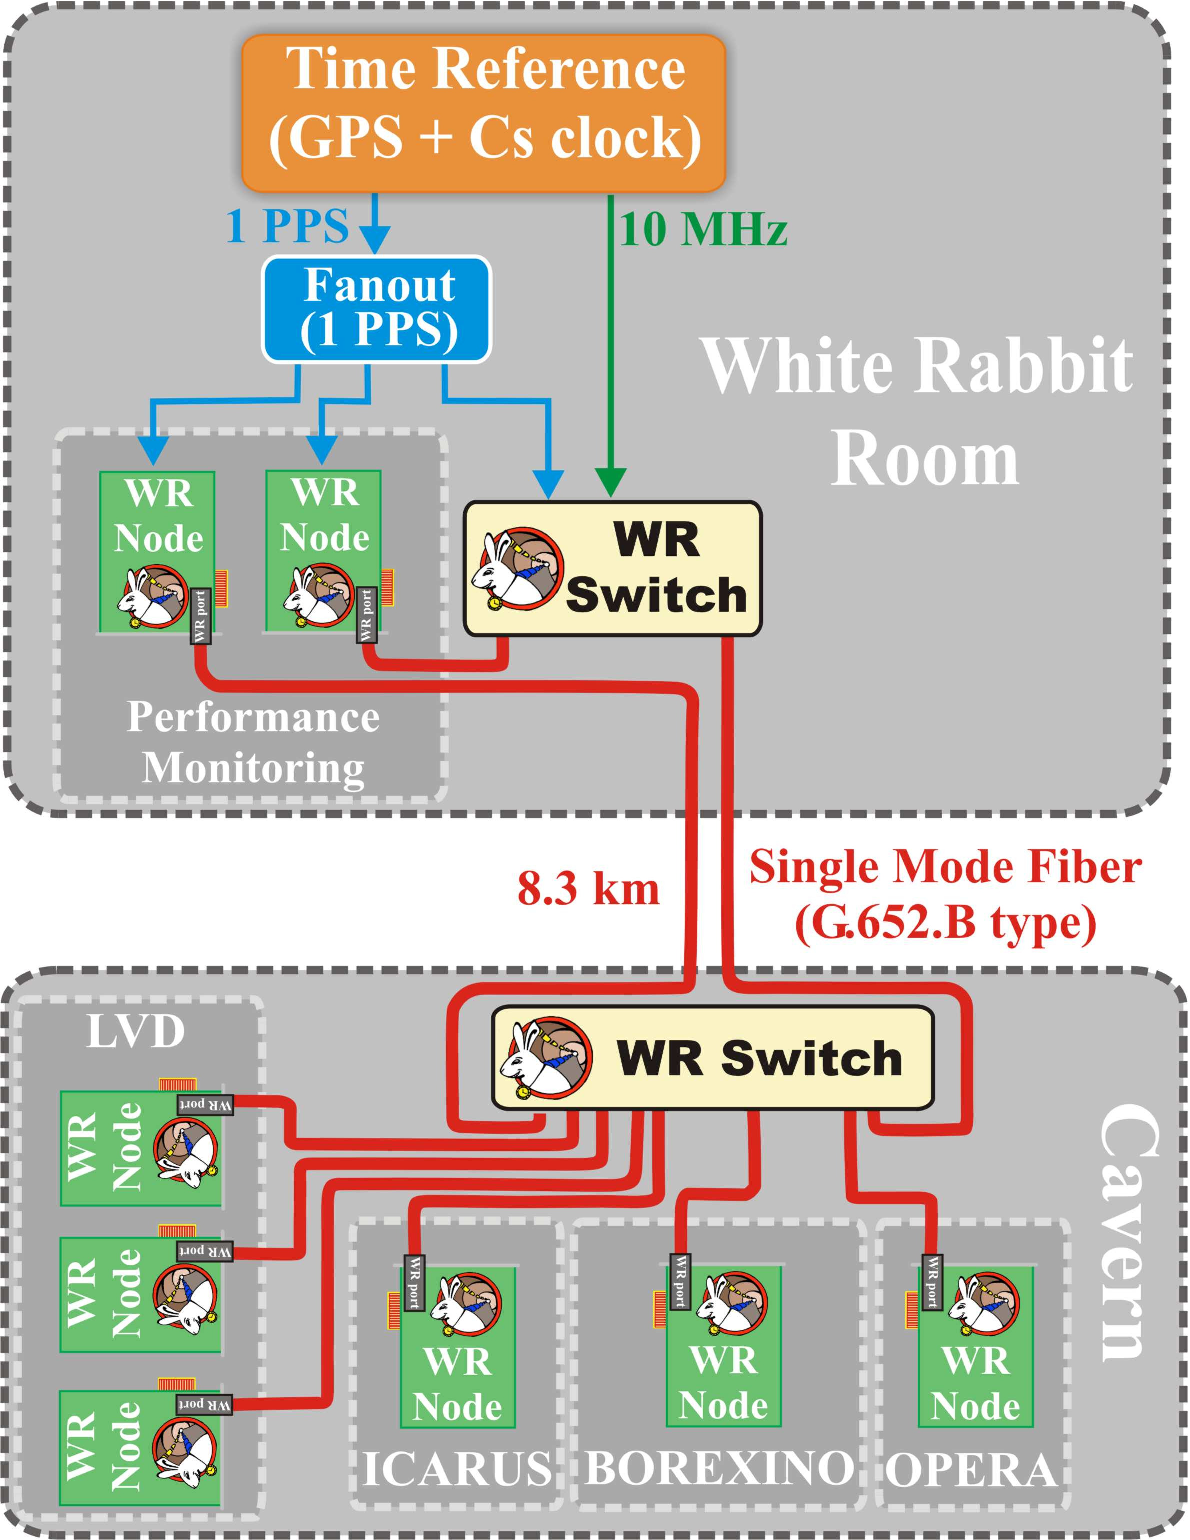
\includegraphics[height=0.75\textheight]{applications/lngs_installation.pdf}
    \end{center}
  \end{columns}
  }

\end{frame}

\begin{frame}{Other WR Applications}

\begin{columns}[c]
  \column{0.7\textwidth}
     \begin{itemize}
         \item<1-> \color<2->{black!50}{CERN and GSI}
         \item<2-> \color<3->{black!50}{HiSCORE: Gamma\&Cosmic-Ray experiment}
         \item<3-> \color<4->{black!50}{The Large High Altitude Air Shower Observatory}
         \item<4-> \color<5->{black!50}{MIKES: Centre for metrology and accreditation}
         \item<5-> {KM3NET: European deep-sea research infrastructure}
     \end{itemize}

    \column{0.45\textwidth}         

    \begin{center}
      \includegraphics<1>[width=0.80\textwidth]{applications/gsiANDcern.pdf}   \pause
      \includegraphics<2>[width=1\textwidth]{applications/tunka.pdf}        \pause
      \includegraphics<3>[width=1\textwidth]{applications/lhaaso.pdf}       \pause
      \includegraphics<4>[width=.7\textwidth]{applications/mikes.pdf}       \pause
      \includegraphics<5>[width=1\textwidth]{applications/KM3NeT.pdf}
   \end{center}

\end{columns}
{\small Full list of WR users: \url{http://www.ohwr.org/projects/white-rabbit/wiki/WRUsers}}

\end{frame}

%%%%%%%%%%%%%%%%%%%%%%%%%%%%%%%%%%%%%%%%%%%%%%%%%%%%%%%%%%%%%%%%%%%%%%%%%%%%%%%%%%%%%%%%%%%%%%%%%%%%
\section{Summary}
\subsection{}
%%%%%%%%%%%%%%%%%%%%%%%%%%%%%%%%%%%%%%%%%%%%%%%%%%%%%%%%%%%%%%%%%%%%%%%%%%%%%%%%%%%%%%%%%%%%%%%%%%%%
\begin{frame}<beamer>{Outline}
    \tableofcontents [currentsection]
\end{frame}
%%%%%%%%%%%%%%%%%%%%%%%%%%%%%%%%%%%%%%%%%%%%%%%%%%%%%%%%%%%%%%%%%%%%%%%%%%%%%%%%%%%%%%%%%%%%%%%%%%%%
\begin{frame}{White Rabbit Family}

    \begin{center}
      Successful international collaboration of institutes, universities and companies
    \end{center}             
    \begin{center}
      \includegraphics<1>[width=1.0\textwidth]{misc/wr_family_1.pdf}
      \includegraphics<2>[width=1.0\textwidth]{misc/wr_family_2.png}
    \end{center}

    \begin{center}
      WR Users: \url{http://www.ohwr.org/projects/white-rabbit/wiki/WRUsers}
    \end{center}  

\end{frame}

%%%%%%%%%%%%%%%%%%%%%%%%%%%%%%%%%%%%%%%%%%%%%%%%%%%%%%%%%%%%%%%%%%%%%%%%%%%%%%%%%%%%%%%%%%%%%%%%%%%%
\begin{frame}{Pushing frontiers}

    \begin{itemize}
	\item<1-> Scientific, open (H/W \& S/W), with commercial support\pause
	\item<2-> More applications than ever expected \pause
	\item<3-> A versatile solution for general control and data acquisition \pause
	\item<4-> Fulfilling all our needs in synchronization and determinism \pause
	\item<5-> Standard-compatible and standard-extending \pause
	\item<6-> Active participation in IEEE1588 revision process\pause
    \end{itemize}  

\end{frame}

%%%%%%%%%%%%%%%%%%%%%%%%%%%%%%%%%%%%%%%%%%%%%%%%%%%%%%%%%%%%%%%%%%%%%%%%%%%%%%%%%%%%%%%%%%%%%%%%%%%%
\subsection*{}
%%%%%%%%%%%%%%%%%%%%%%%%%%%%%%%%%%%%%%%%%%%%%%%%%%%%%%%%%%%%%%%%%%%%%%%%%%%%%%%%%%%%%%%%%%%%%%%%%%%%
\begin{frame}{Thank you}

    \begin{center}
    
\includegraphics[height=4.0cm]{misc/white_rabbit_end.png}
    \end{center}

   \begin{center}

      More information: \\
      http://www.ohwr.org/projects/white-rabbit/wiki
    \end{center}  

\end{frame}

%%%%%%%%%%%%%%%%%%%%%%%%%%%%%%%%%%%%%%%%%%%%%%%%%%%%%%%%%%%%%%%%%%%%%%%%%%%%%%%%%%%%%%%%%%%%%%%%%%%%
%%%%%%%%%%%%%%%%%%%%%%%%%%%%%%%%%%%%%%%%%%%%%%%%%%%%%%%%%%%%%%%%%%%%%%%%%%%%%%%%%%%%%%%%%%%%%%%%%%%%

\appendix

\backupbegin

\section{Even more stuff...}
\subsection{}

\begin{frame}{Link Delay Model}
 \begin{center}
 \includegraphics<1>[height=4cm]{protocol/wrLinkModel_1.pdf}
 \includegraphics<2>[height=4cm]{protocol/wrLinkModel_init.pdf}
 \end{center}
\end{frame}

\begin{frame}{Link Delay Model}
 \begin{align}
   \nonumber delay_{ms} &= \Delta_{tx_m} + \delta_{ms} + \Delta_{rx_s} \\
   \nonumber delay_{sm} &= \Delta_{tx_s} + \delta_{sm} + \Delta_{rx_m}
 \end{align}

  \vspace{0.2cm}

 \begin{center}
 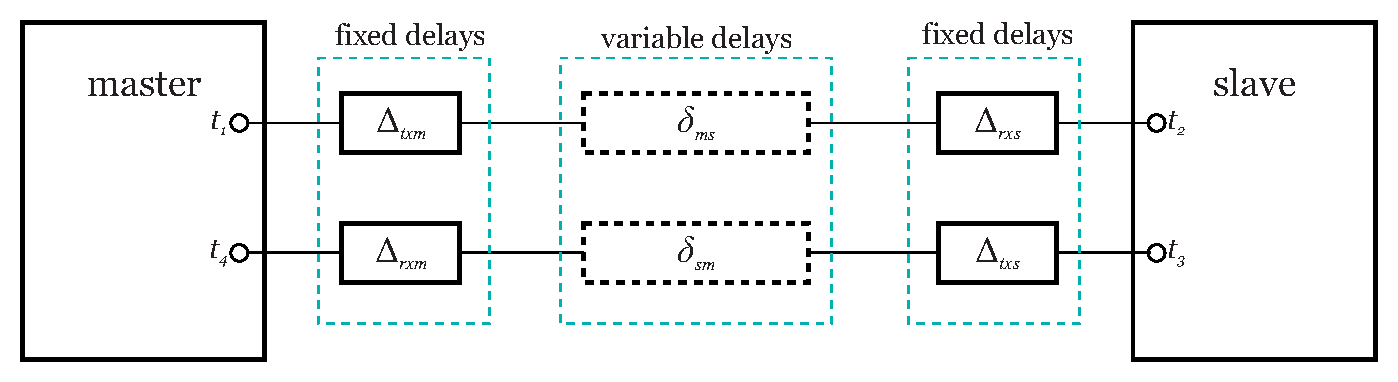
\includegraphics[height=2.5cm]{protocol/delaymodel.pdf}
 \end{center}

 \only<2> {
 \begin{columns}[c]
   \column{2.8in}
 
     \begin{center}
       \textbf{Relative Delay Coefficient ($\alpha$)} \\
       for 1000base-X over a Single-mode Optical Fibre
     \end{center}
 
   \column{1.5in}
     \begin{center}
       \begin{equation}
       \nonumber \delta_{ms} = (1 + \alpha) \, \delta_{sm}
       \end{equation}
     \end{center}
     \vspace{0.5cm}
 \end{columns}}

 \onslide<3> {
 \begin{block}{Measuring fixed delays is hard}
 	but we use mathematical tricks for that - \emph{WR Calibration procedure} (\url{http://www.ohwr.org/documents/213})
 \end{block}}

\end{frame}

\begin{frame}{White Rabbit extension to PTP}

\begin{columns}[c]
  \column{0.7\textwidth}
    \begin{itemize}
	\item White Rabbit requires:
	  \begin{itemize}
	    \item WR-specific states
	    \item Exchange of WR-specific information
      \item asymmetry estimation based on Link Delay Model
	  \end{itemize}
	\item WR PTP
	  \begin{itemize}
	    \item PTP extensions mechanisms
	    \item Enhanced precision $t_1$, $t_2$, $t_3$, $t_4$
	    \item Correction for asymmetry
	    \item Interoperability with PTP gear
	  \end{itemize}
  \end{itemize}
  \column{0.3\textwidth}
	\begin{center}
	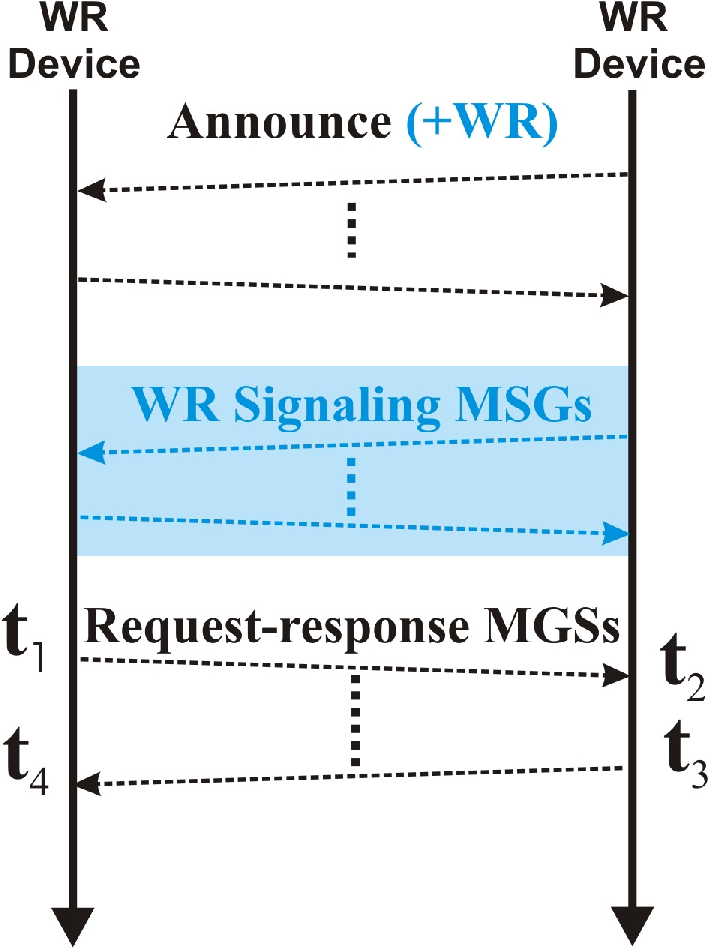
\includegraphics[width=1.1\textwidth]{protocol/wr-ptp-exchange.pdf}
	\end{center}
\end{columns}

\end{frame}

\begin{frame}{White Rabbit Network}
    \begin{itemize}
      \item White Rabbit Switch
      \item White Rabbit Node (White Rabbit PTP Core)
    \end{itemize}
    \begin{center}
    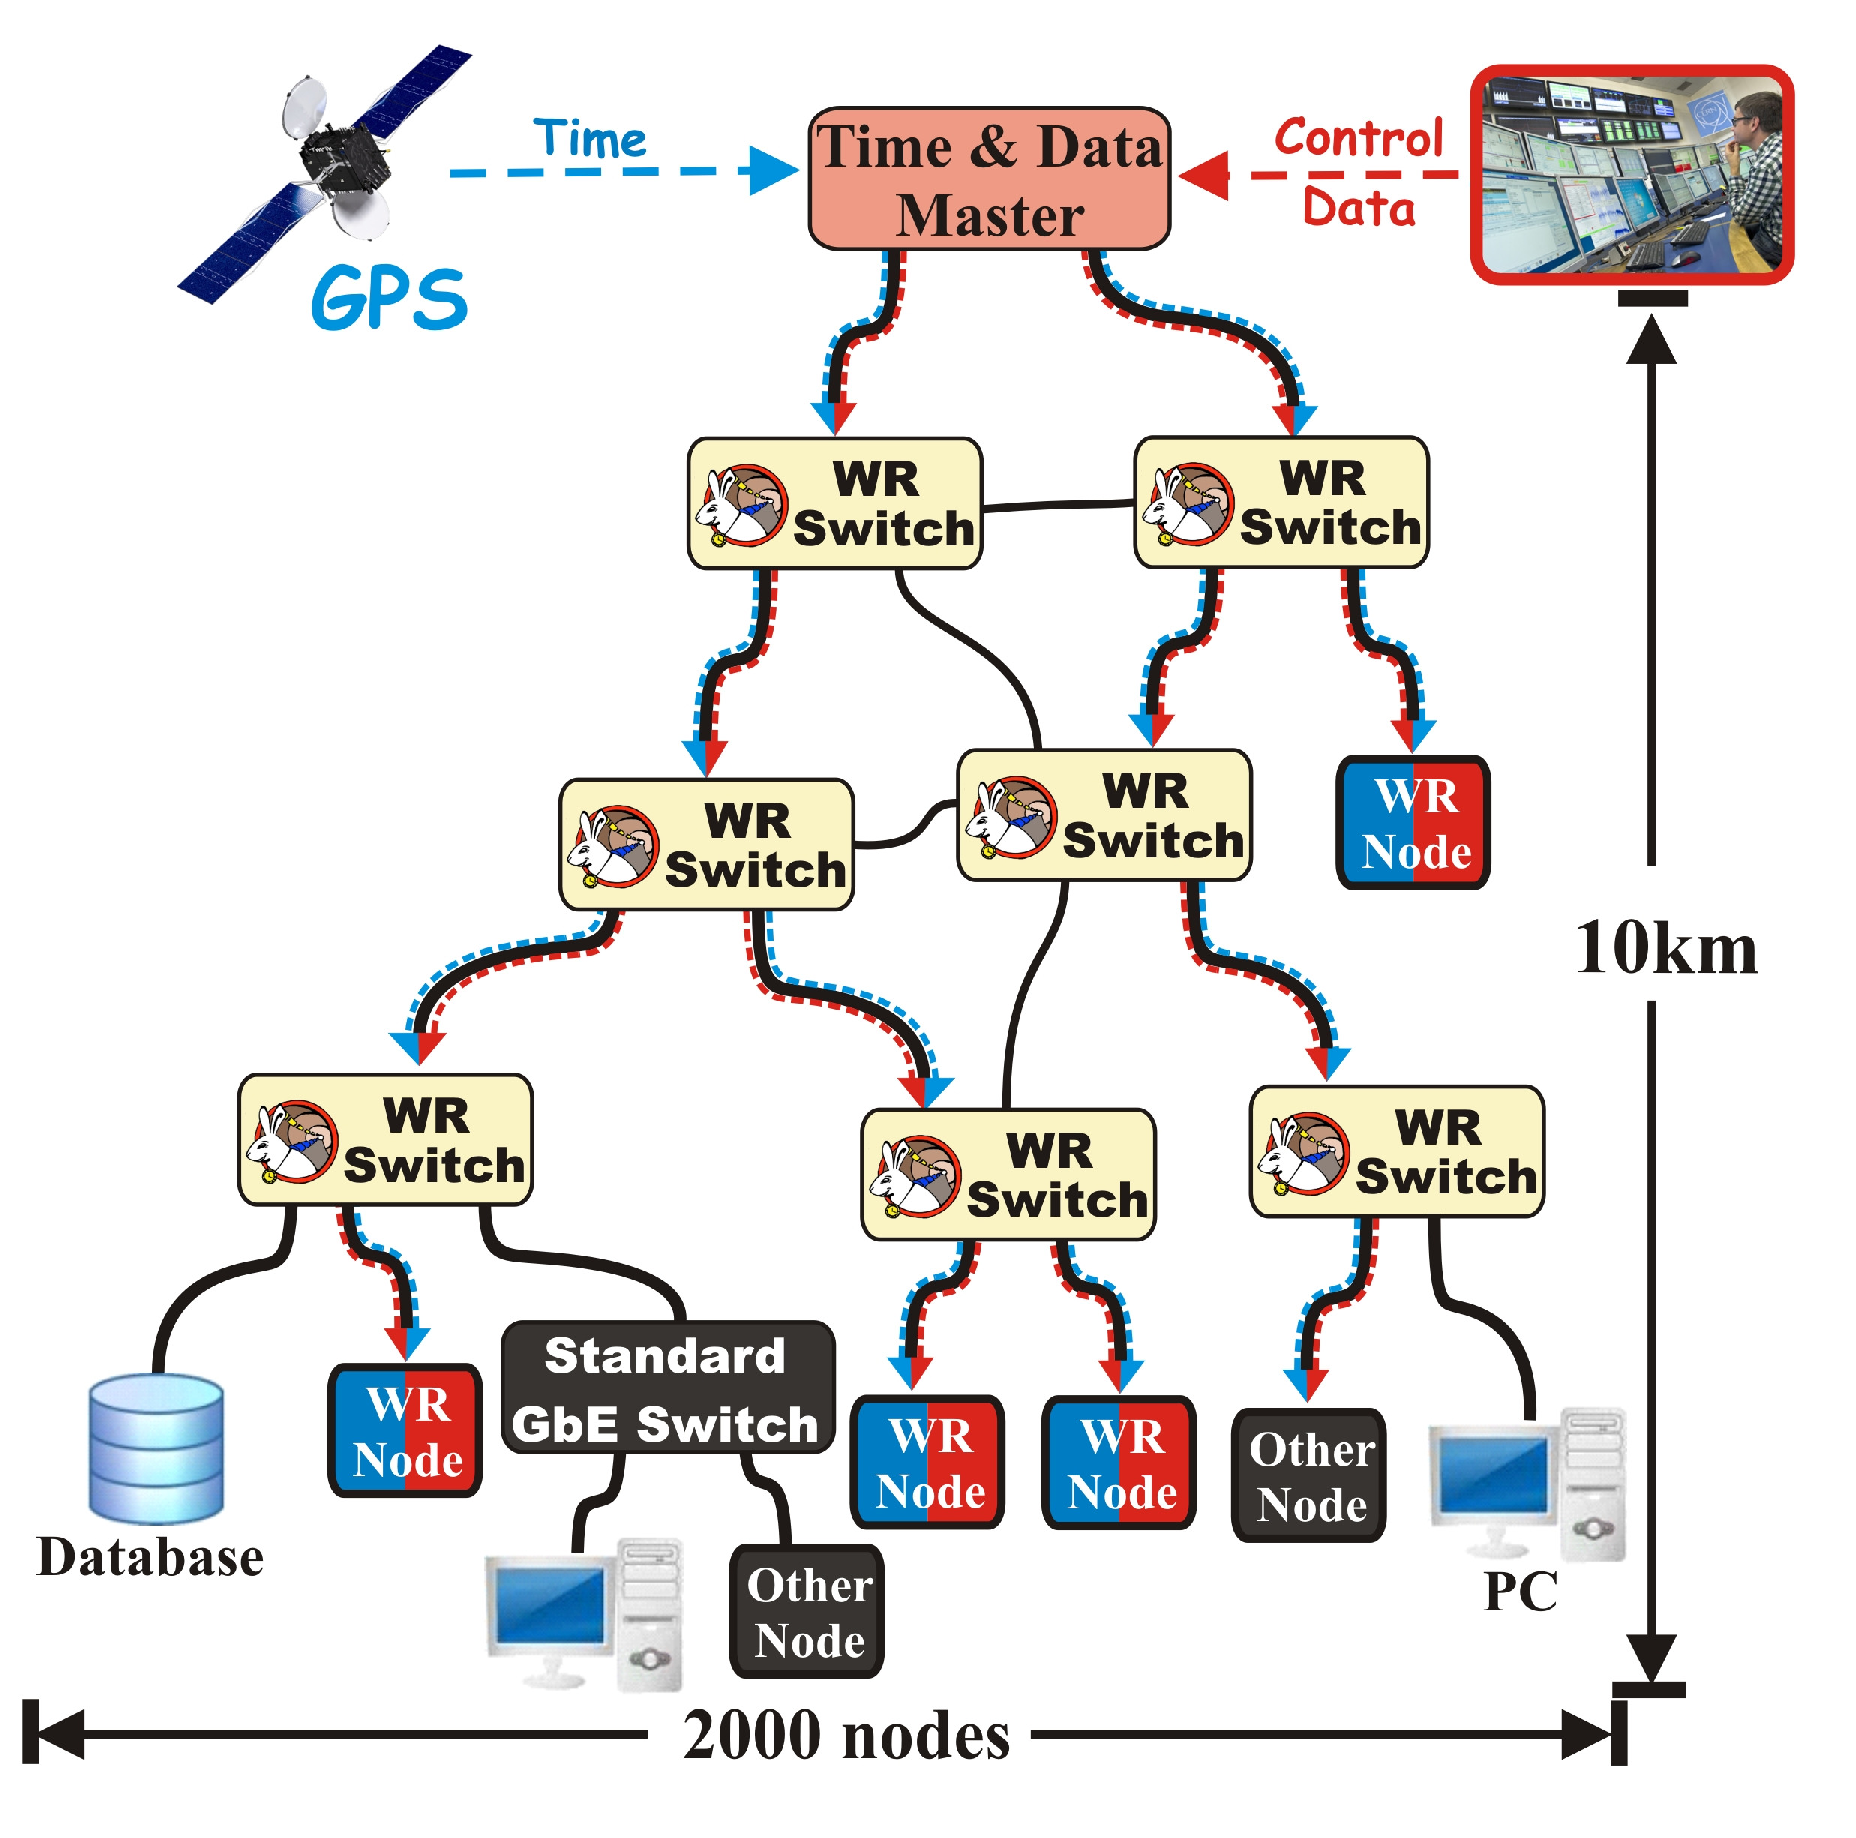
\includegraphics[width=.5\textwidth]{network/wr_network-enhanced_pro.pdf}
    \end{center}
\end{frame}

\begin{frame}{White Rabbit Switch}
	\begin{block}{Functionality of a professional Gigabit Ethernet Switch}
	with White Rabbit extensions
	\end{block}
	\begin{block}{3 layers of design:}
	\begin{center}
	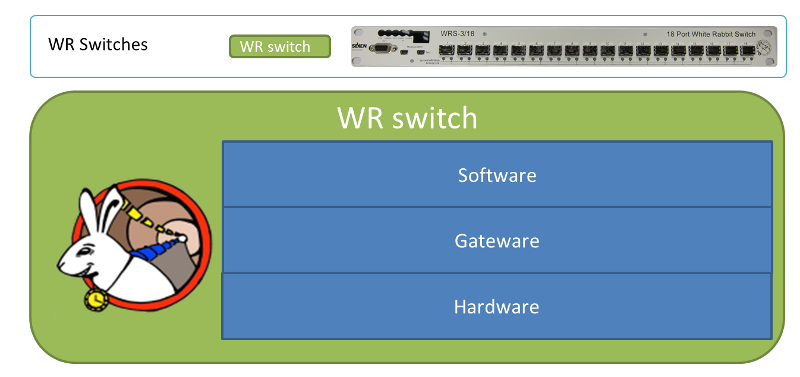
\includegraphics[width=\textwidth]{switch/wrSwitch.png}
	\end{center}
	\end{block}
\end{frame}

\begin{frame}{WR Switch: hardware}
	\begin{center}
	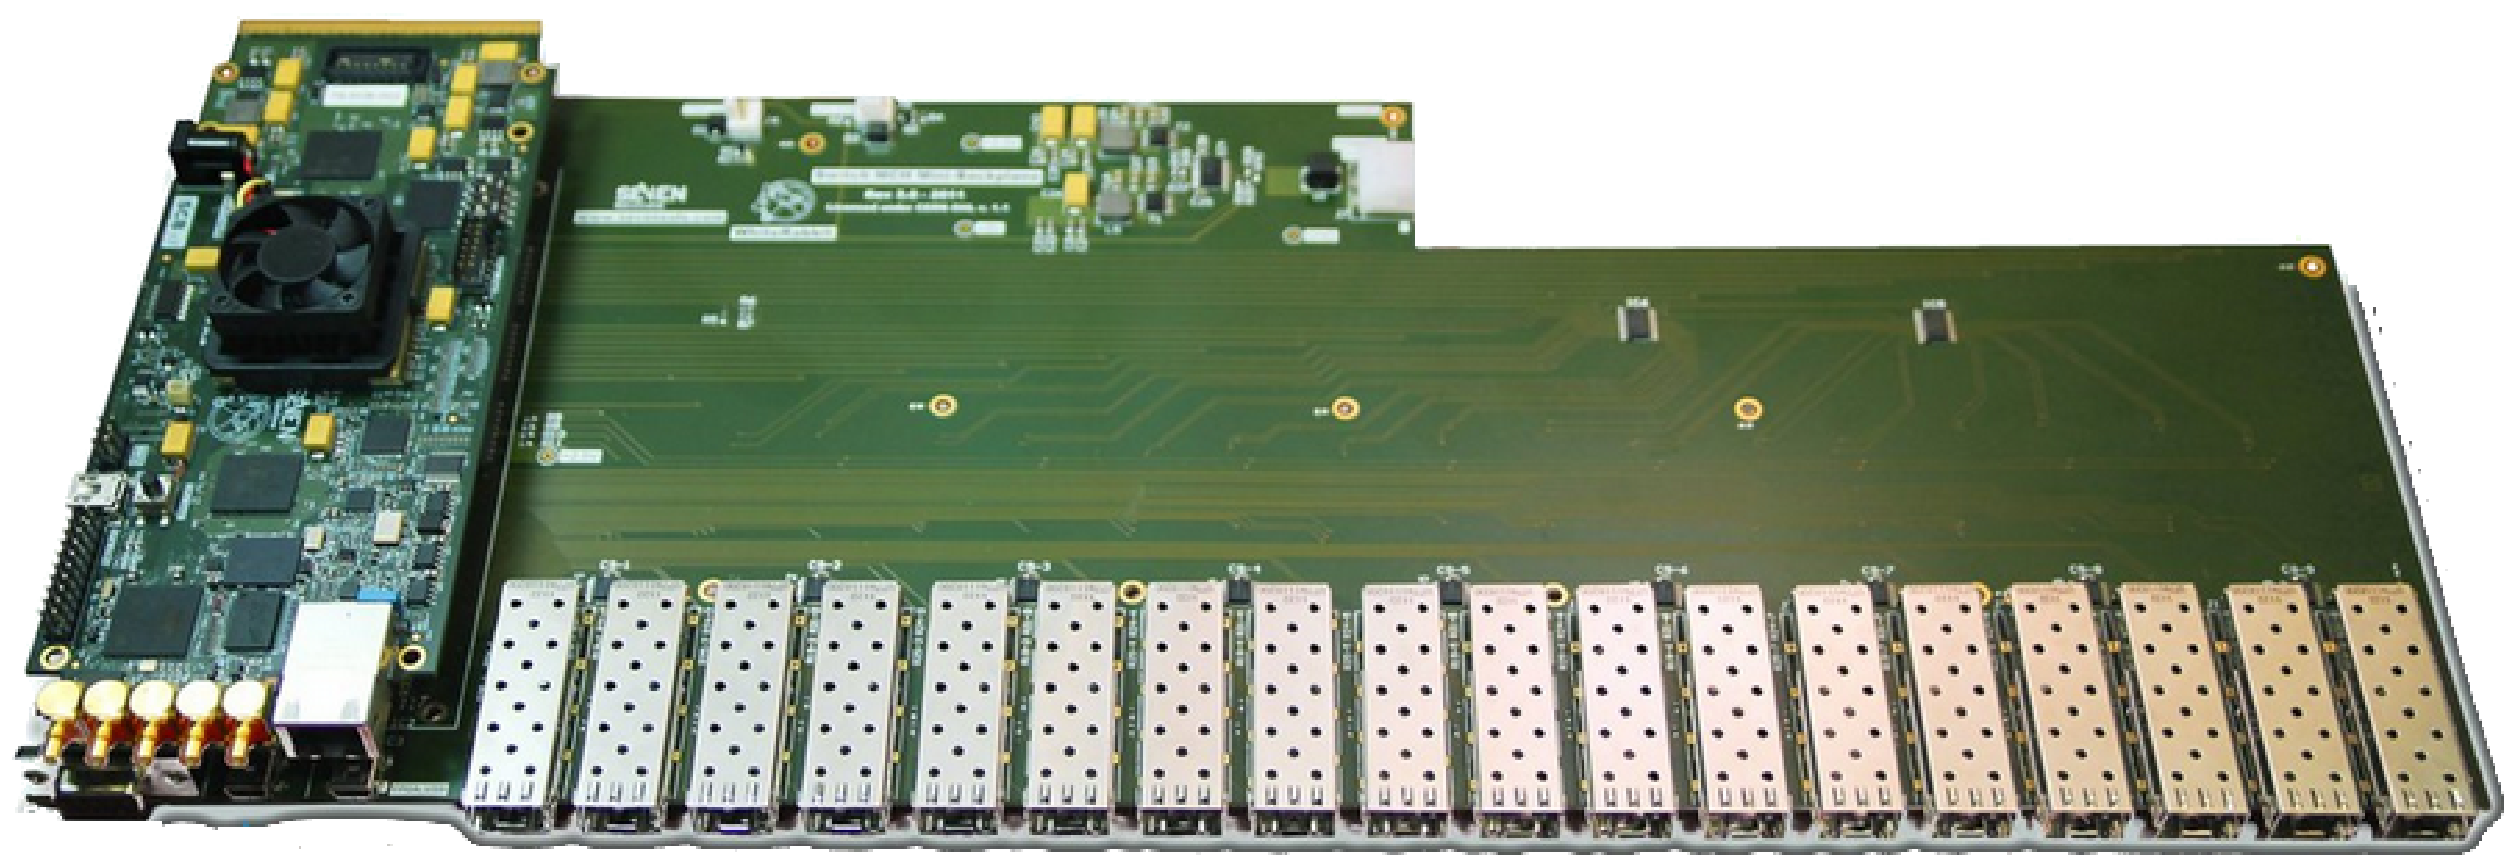
\includegraphics[width=.7\textwidth]{switch/scb_backplane.png}
	\end{center}
	\begin{itemize}
	\item Xilinx Virtex 6, Atmel AT91SAM9G45
	\item 18 cages for Gigabit SFPs, 10/100 Ethernet management port
	\item 5 SMC connectors (1-PPS in/out, CLK in/out)
	\item designed and produced by \emph{Seven Solutions} in cooperation with CERN
	\end{itemize}
\end{frame}

\begin{frame}{WR Switch: gateware}
	Implemented in Xilinx Virtex6 FPGA:
	\begin{center}
	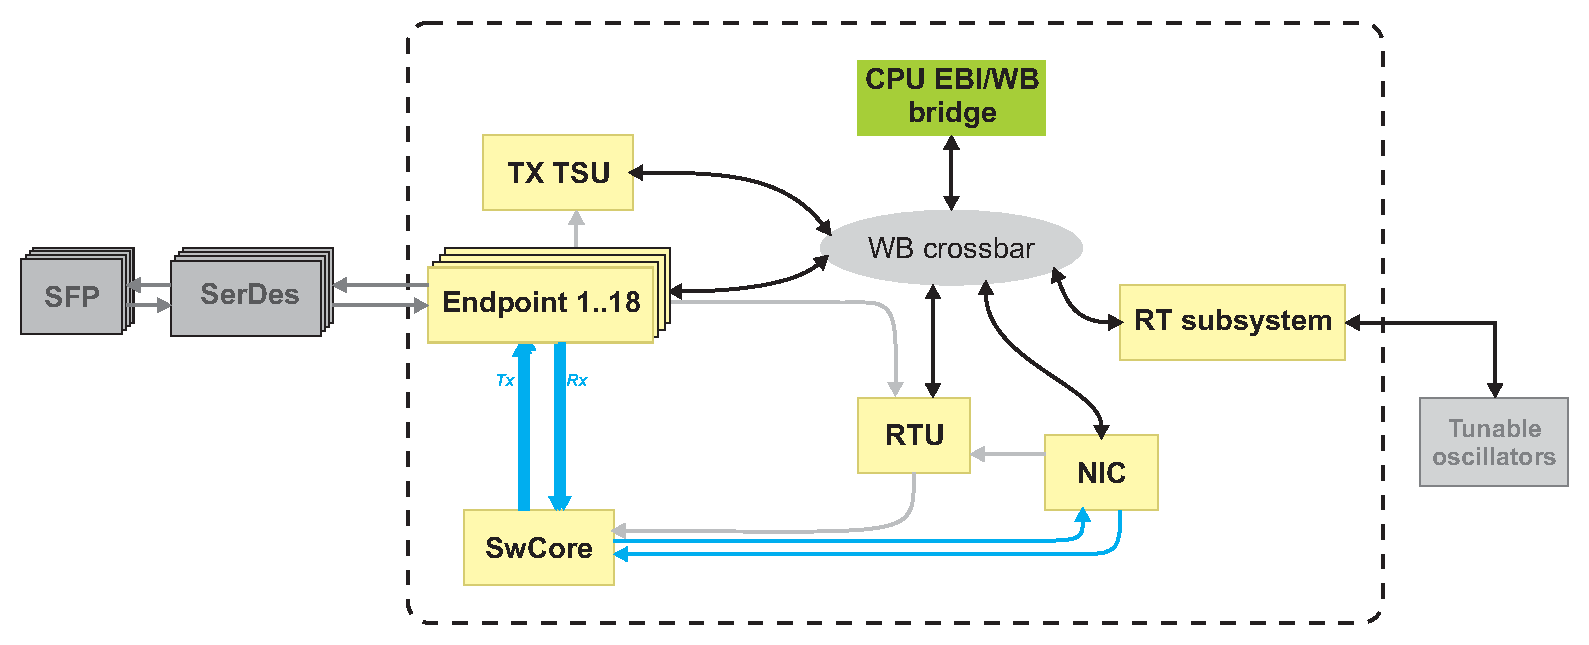
\includegraphics[width=.9\textwidth]{switch/switch_hdl.pdf}
	\end{center}
\end{frame}

\begin{frame}{WR Switch: software}
	Running on ARM processor:
	\begin{itemize}
	\item Embedded Linux
	\item kernel 2.6.39 with patches and modules for HDL components
	\item Hardware Abstraction Layer
	\item RTU daemon
	\item PTP daemon with WR extension
	\item CLI and SNMP support coming
	\end{itemize}
\end{frame}

\begin{frame}{White Rabbit Node - WR PTP Core}
	\begin{block}{HDL IP-Core}
	developed on Xilinx Spartan 6 but not tied to Xilinx
	\end{block}
	\begin{block}{it is a fancy Ethernet MAC}
	\begin{itemize}
	\item interfaces user-defined module sending/receiving Ethernet frames with PHY layer
	\item provides precise timing by implementing WR protocol
	\end{itemize}
	\end{block}
	\begin{block}{ready to be integrated in user's devices}
	requires only two tunable oscillators and EEPROM to store the configuration
	\end{block}
\end{frame}

\begin{frame}{WR PTP Core: interfaces}
	\begin{itemize}
		\item clocks and reset
		\item frame interface (WR Fabric)
		\item timecode and 1-PPS output
		\item PHY interface (\emph{GTP}/\emph{GTX} tested and supported)
		\item $I^2C$, 1-Wire, UART, GPIO
	\end{itemize}
	\begin{center}
		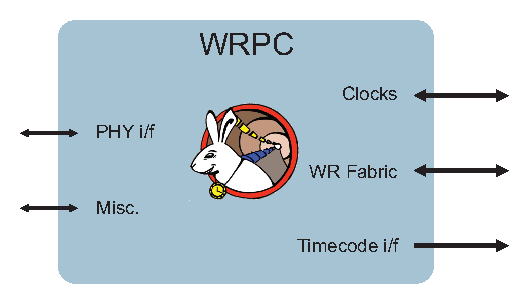
\includegraphics[width=.7\textwidth]{node/wrpc_overview.pdf}
	\end{center}
\end{frame}

\begin{frame}{WR PTP Core: HDL design}
	\begin{center}
	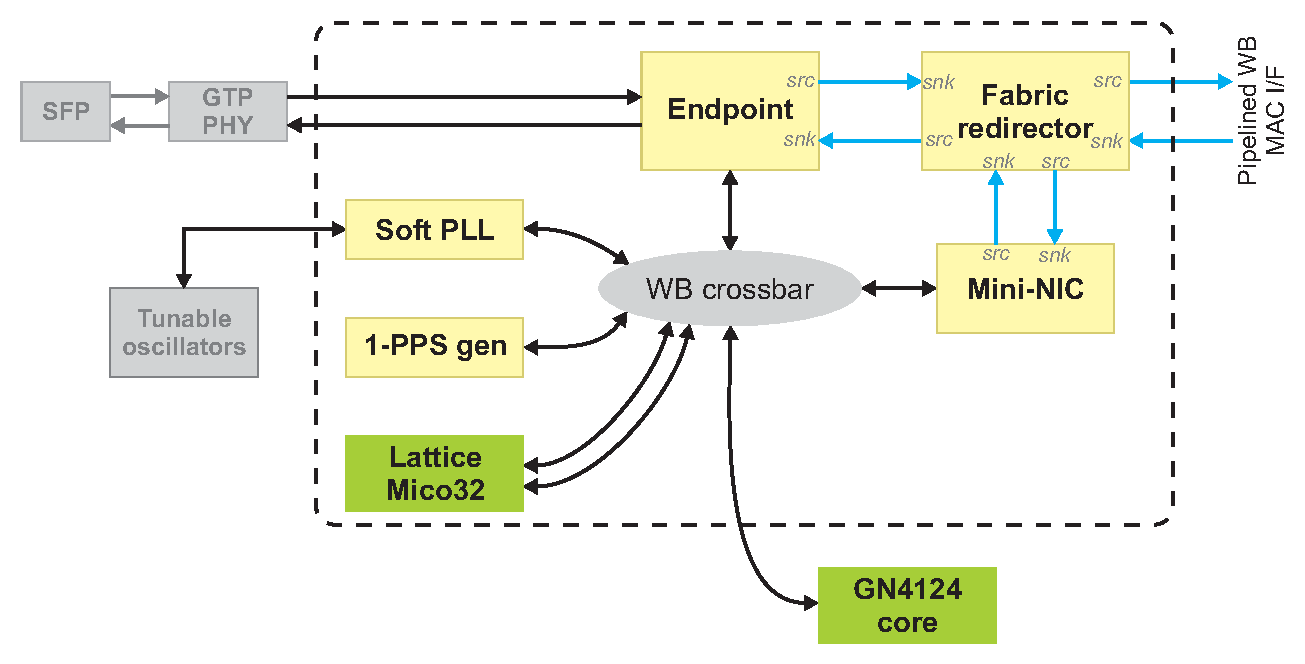
\includegraphics[width=\textwidth]{node/wrpc_inside_simple.pdf}
	\end{center}
\end{frame}
\begin{frame}{WR PTP Core: HDL design}
	\begin{center}
	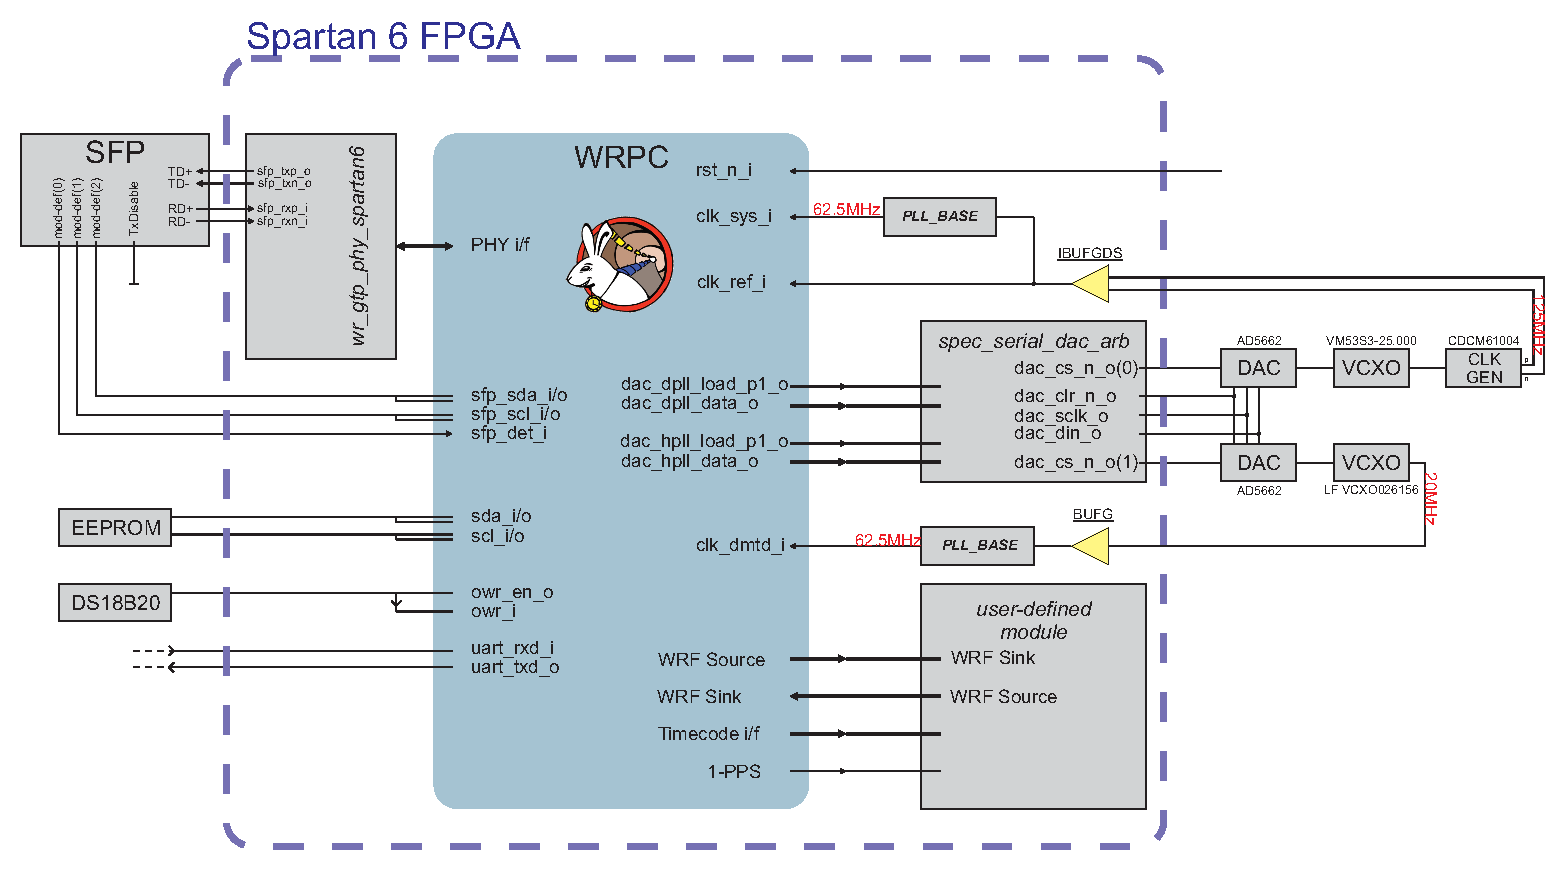
\includegraphics[width=\textwidth]{node/wrpc_basic_top.pdf}
	\end{center}
\end{frame}


\backupend

%%%%%%%%%%%%%%%%%%%%%%%%%%%%%%%%%%%%%%%%%%%%%%%%%%%%%%%%%%%%%%%%%%%%%%%%%%%%%%%%%%%%%%%%%%%%%%%%%%%%%%%%
\end{document}
